\documentclass{article}
\usepackage{hyperref}
\usepackage{amsmath,amssymb}
\usepackage{graphicx}
\usepackage{caption}
\usepackage{subcaption}
\usepackage[section]{placeins}
\renewcommand{\thesubsection}{\thesection.\alph{subsection}}
\usepackage{listings}

\title{\bf{CSE397: Assignment \#1}}
\author{Nicholas Malaya \\ Institute for Computational Engineering and Sciences \\ University of Texas at Austin} \date{}

\begin{document}
\maketitle

\newpage
\section{Problem 1}

\begin{figure}[!htb]
  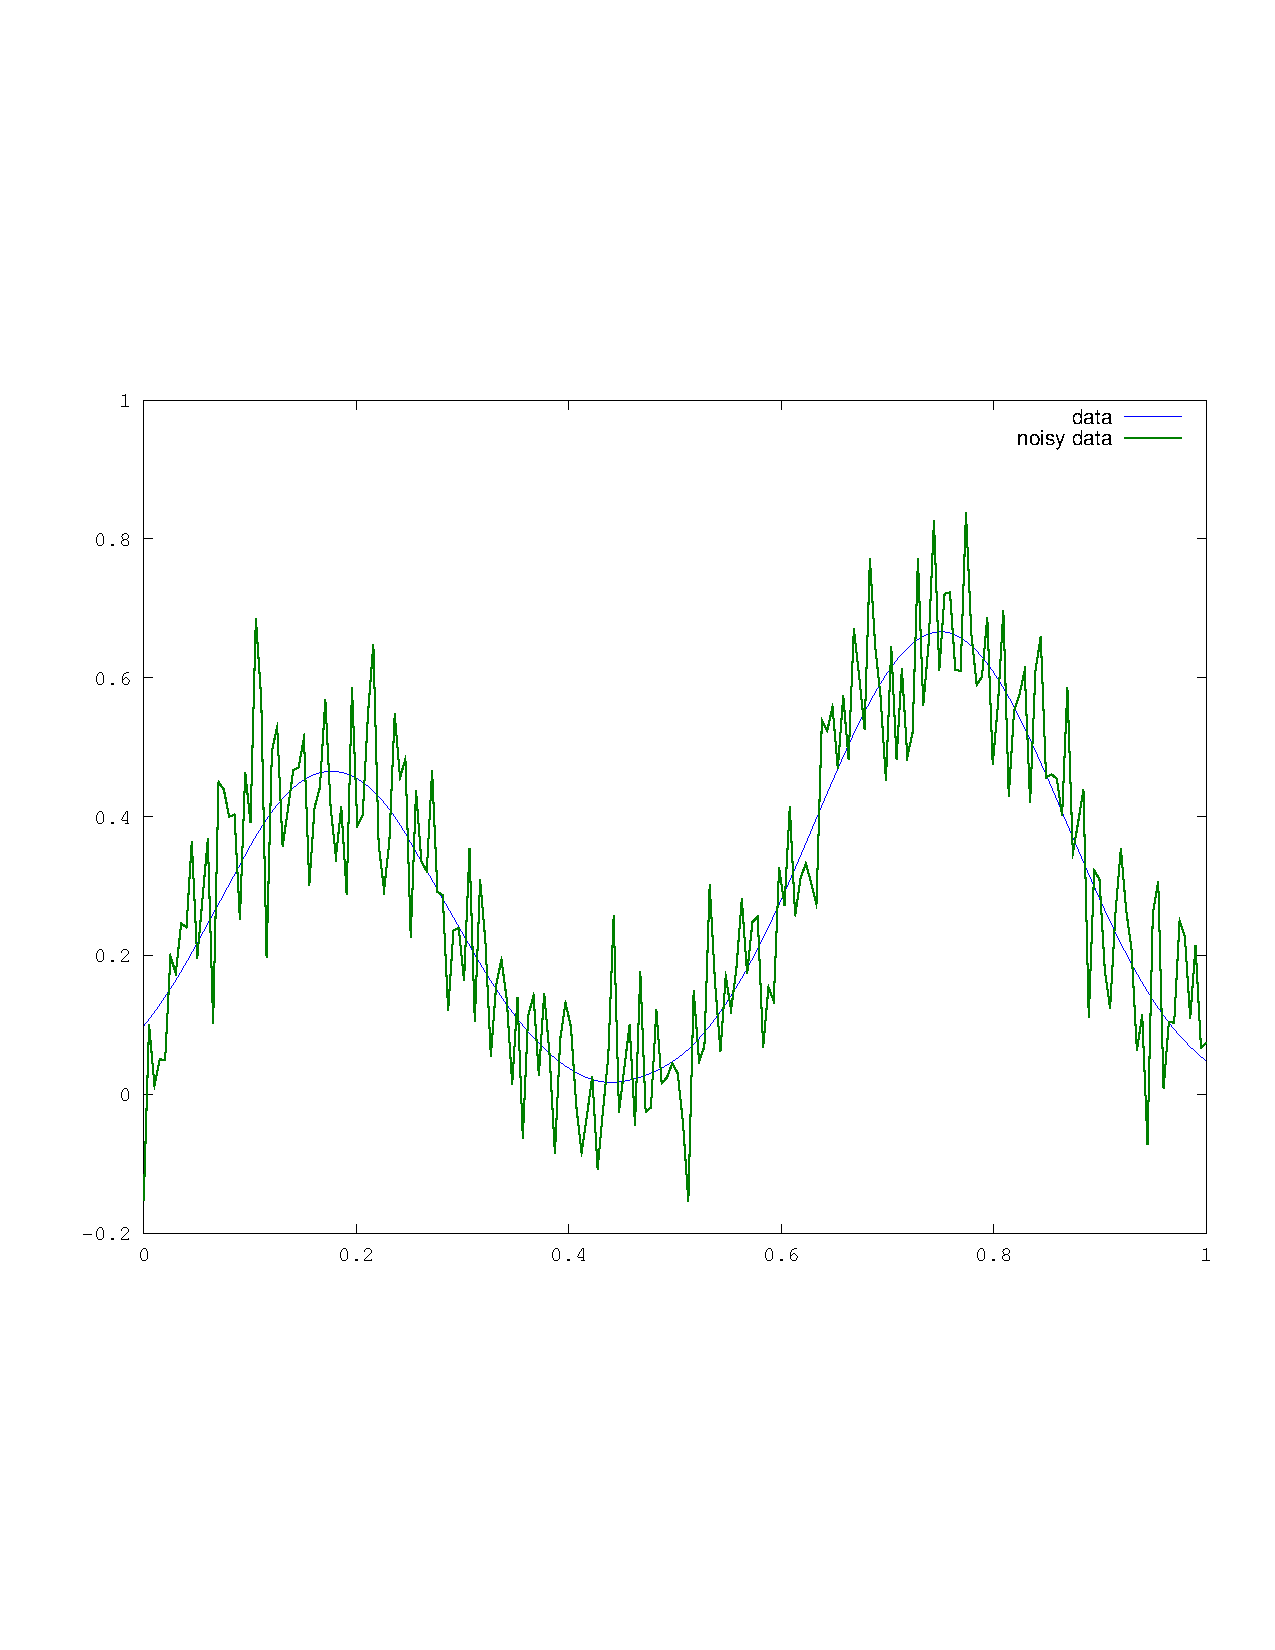
\includegraphics[scale=.5]{plots/data.pdf}
  \label{fig:data}
  \caption{The data (after applying the filter) with and without
 normally distributed noise. } 
\end{figure}

After applying the new filter $k(x)$ and adding gaussian noise, the data
used as input for the inverse problem is plotted in figure 1. 

Notice that this filter is significant: the raw data generated after
passing through the filter (even without statistical noise) has lost
several features of the underlying ``true'' signal. 

\subsection{$T_{\text{SVD}}$}


\begin{figure}[!htb]
        \centering
        \begin{subfigure}[bh]{0.45\textwidth}
                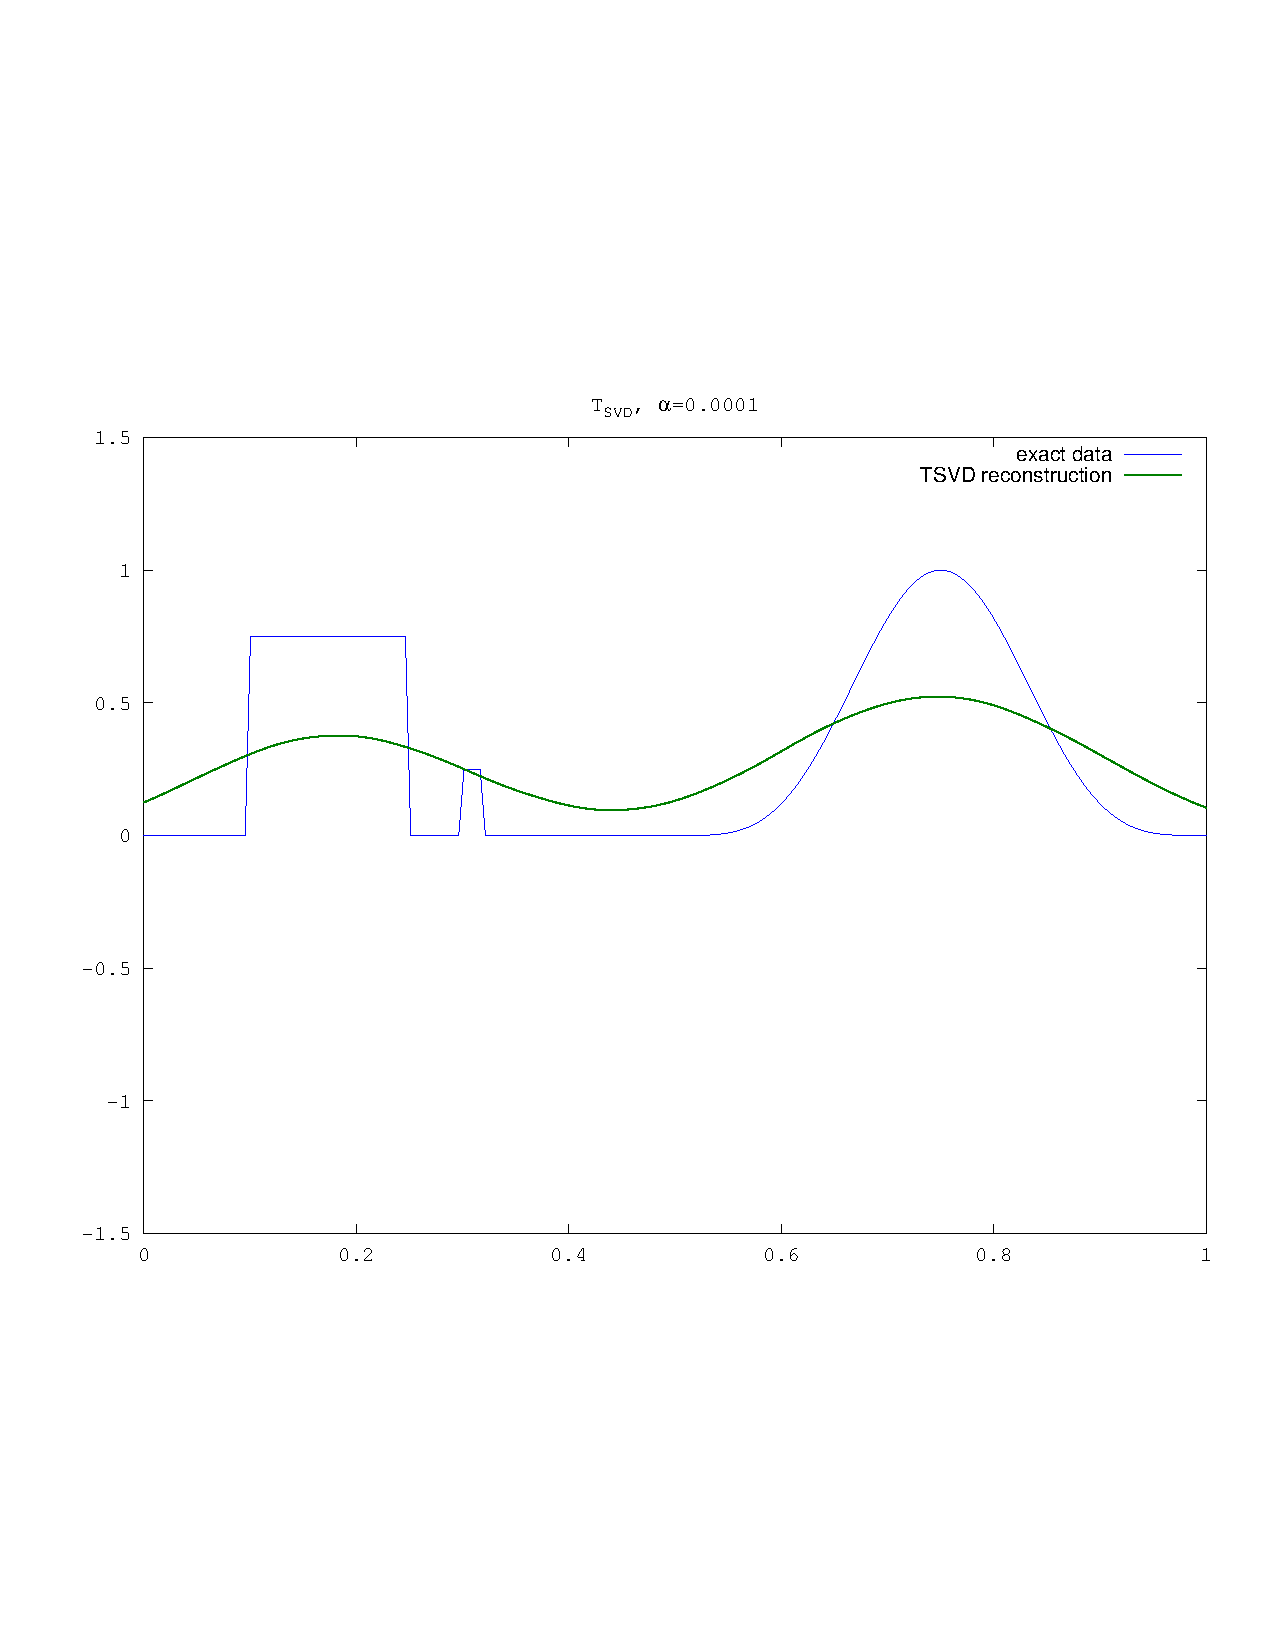
\includegraphics[width=\textwidth]{plots/tsvd0001.pdf}
                \caption{$\alpha=0.0001$}
        \end{subfigure}%
        \begin{subfigure}[bh]{0.45\textwidth}
                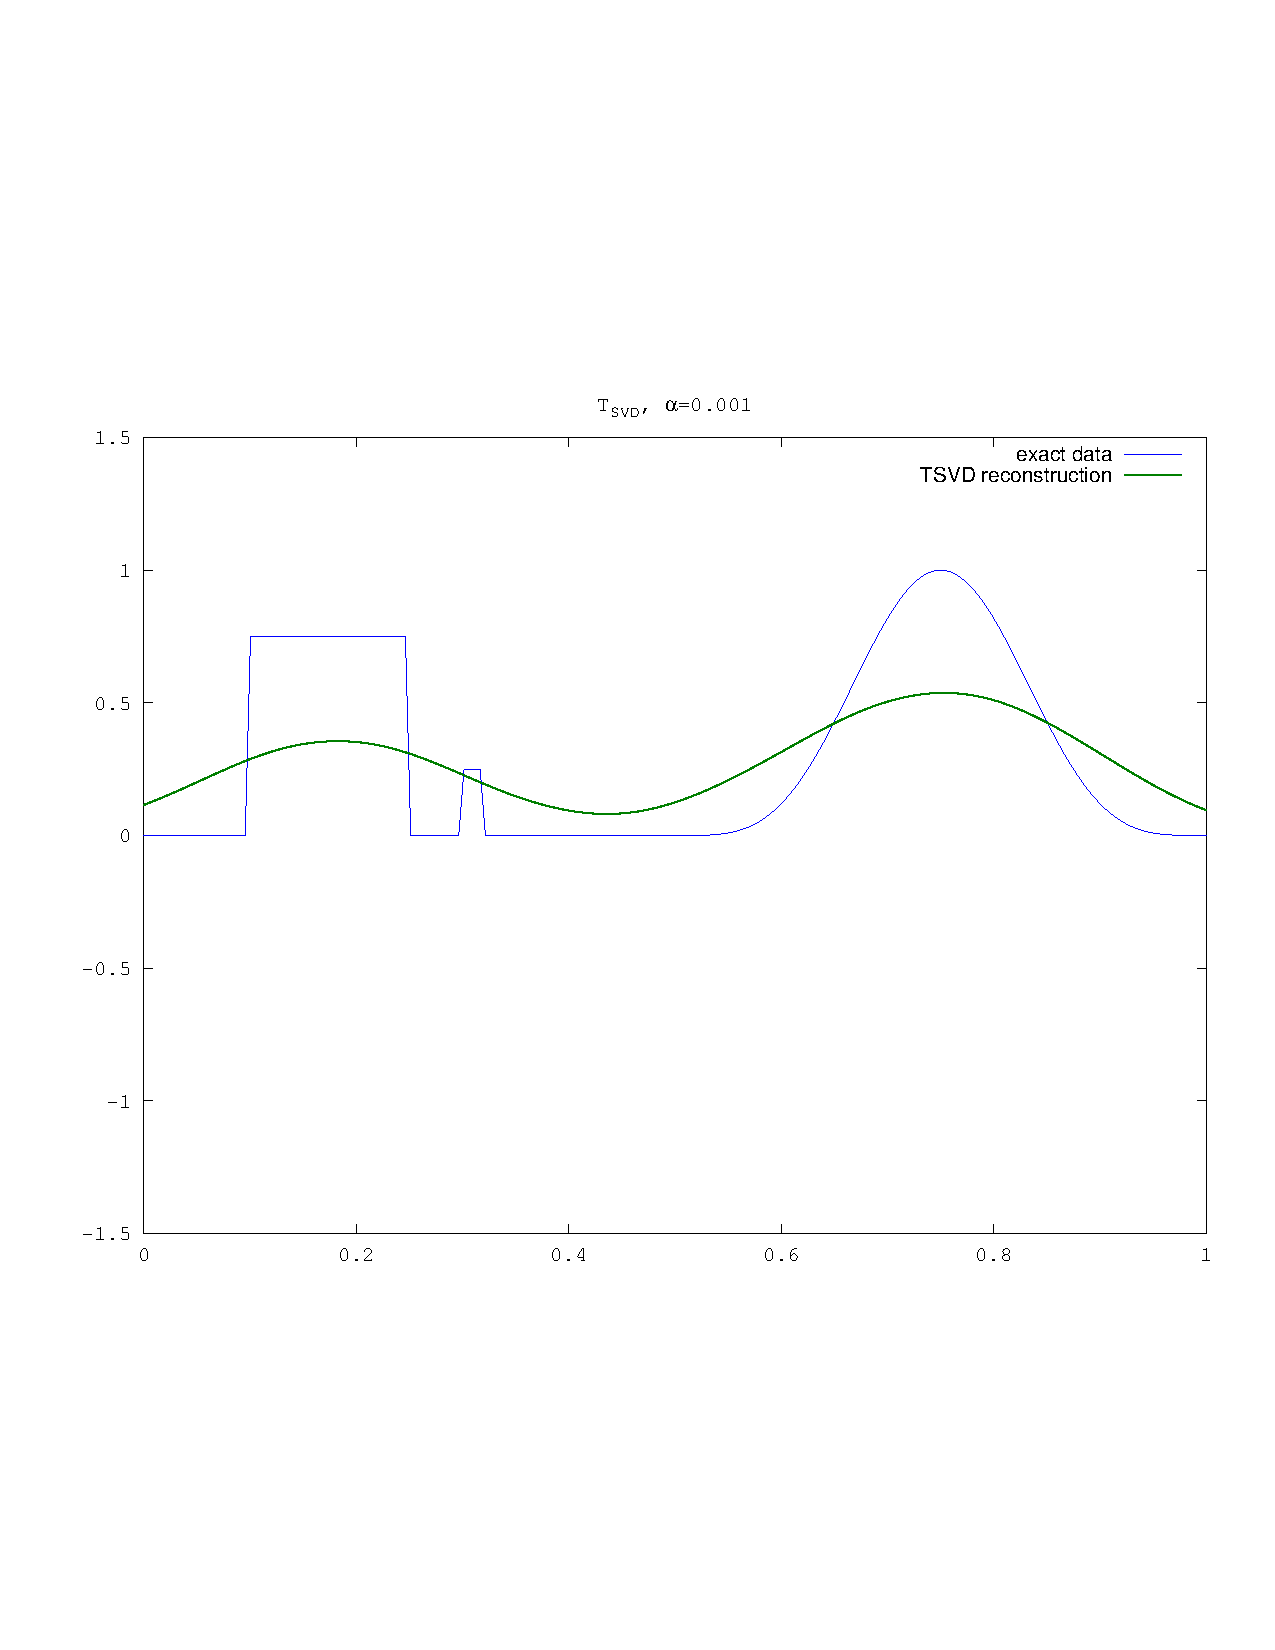
\includegraphics[width=\textwidth]{plots/tsvd001.pdf}
                \caption{$\alpha=0.001$}
        \end{subfigure}
        \centering
        \begin{subfigure}[bh]{0.45\textwidth}
                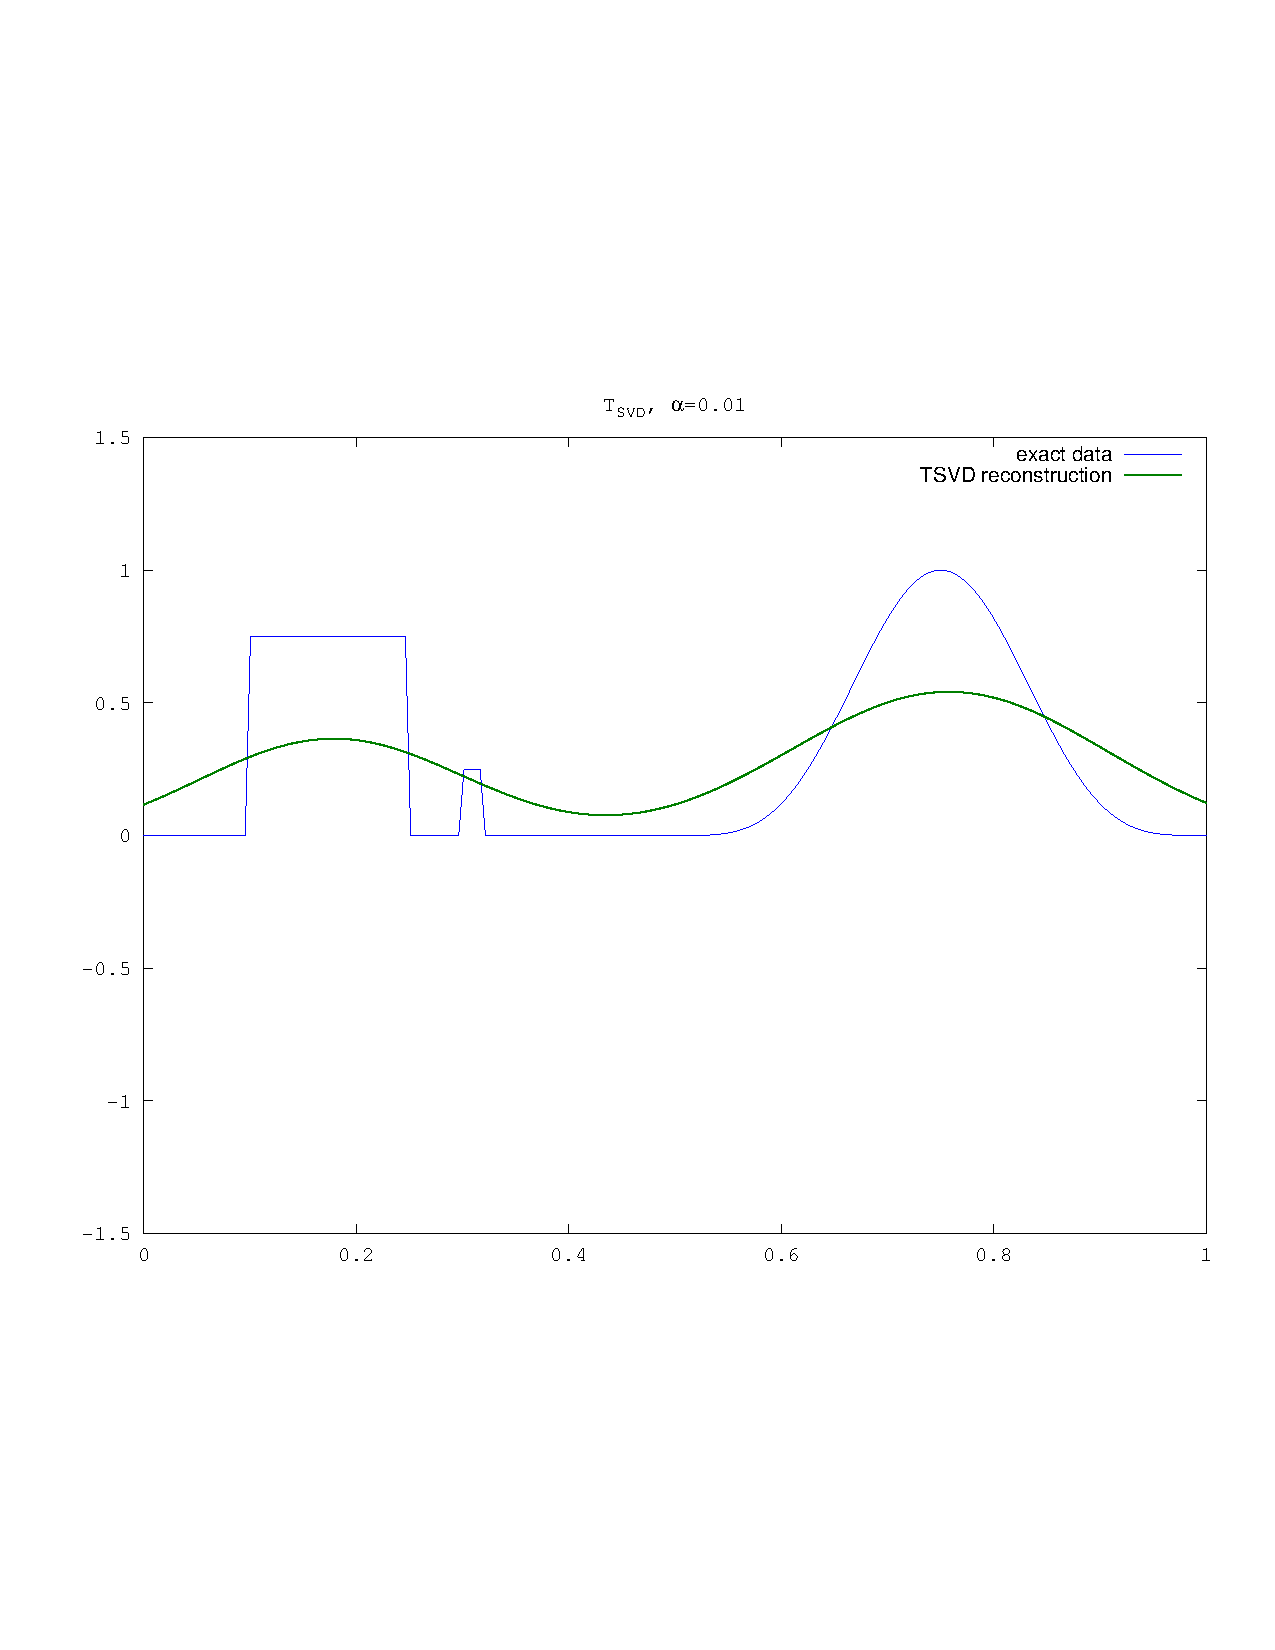
\includegraphics[width=\textwidth]{plots/tsvd01.pdf}
                \caption{$\alpha=0.1$}
        \end{subfigure}%
        \begin{subfigure}[bh]{0.45\textwidth}
                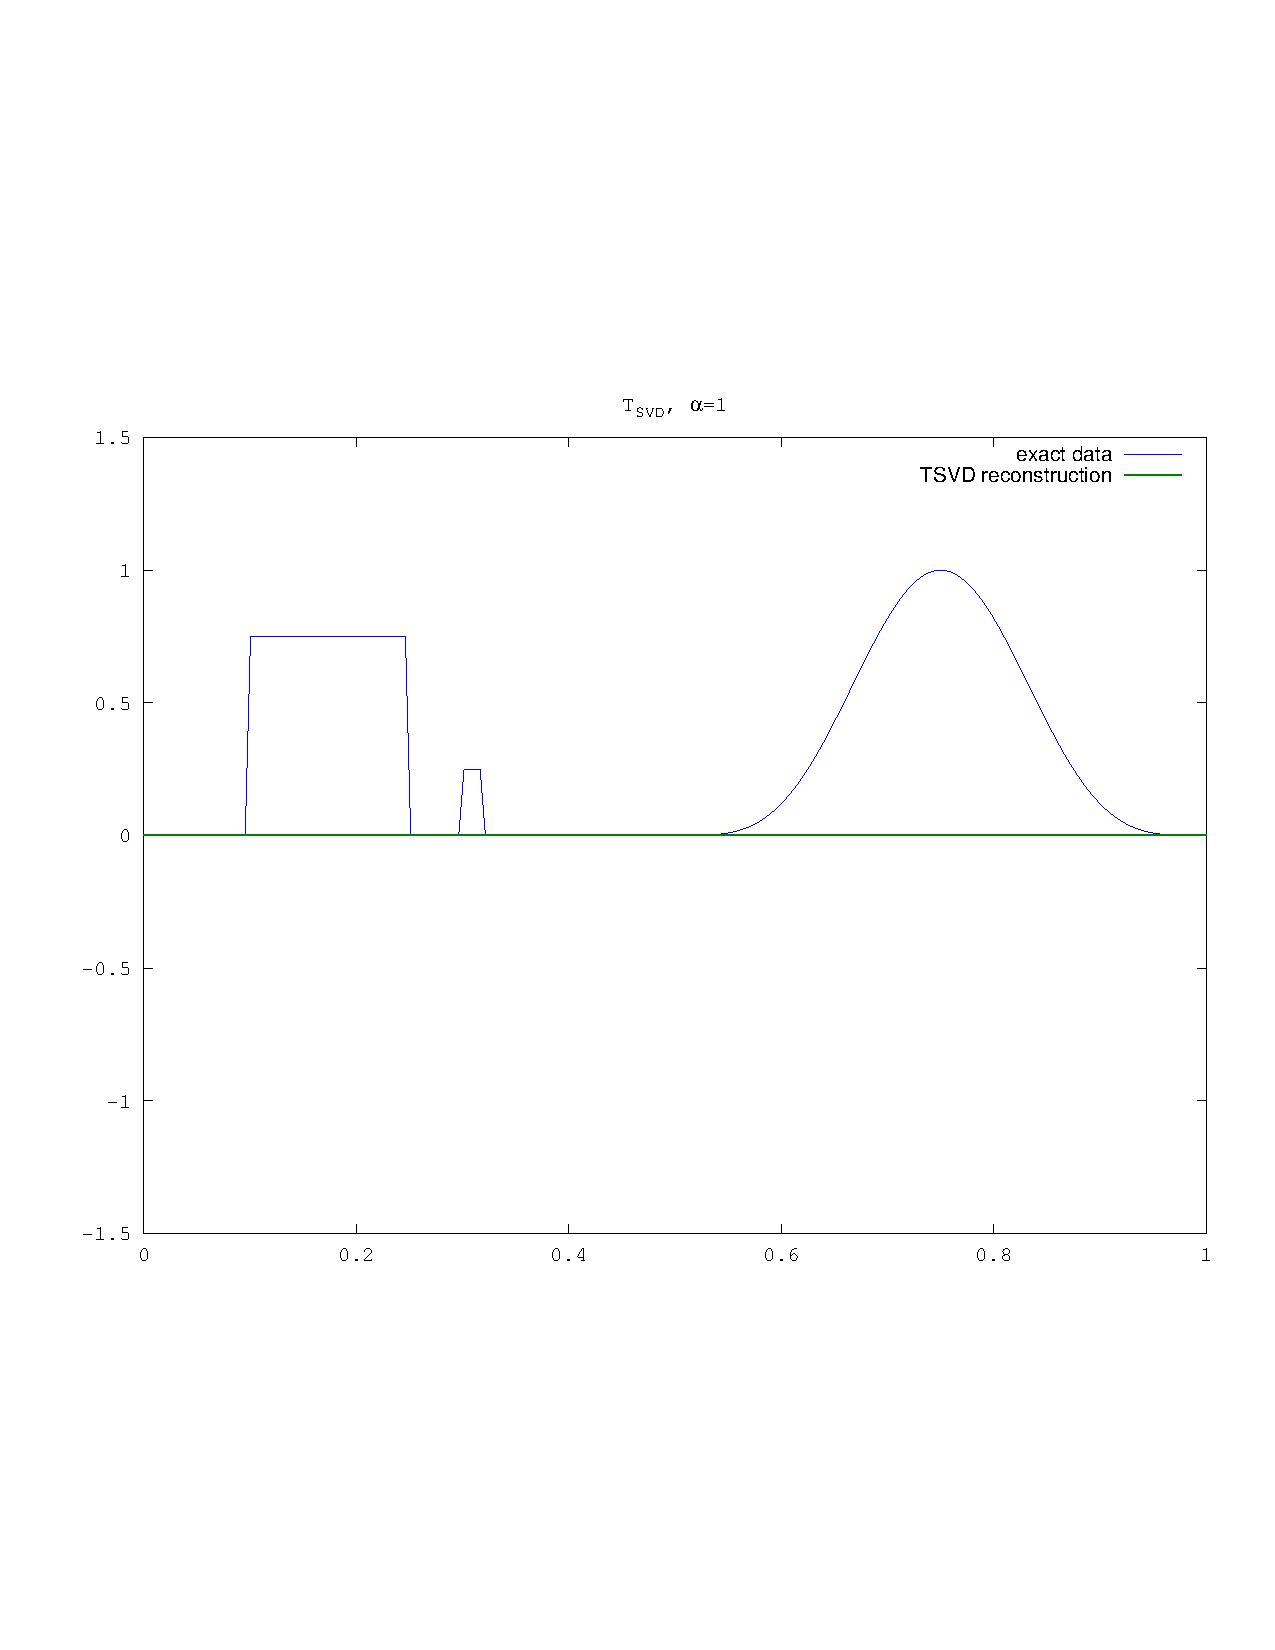
\includegraphics[width=\textwidth]{plots/tsvd1.pdf}
                \caption{$\alpha=1.0$}
        \end{subfigure}
        \caption{$T_{\text{SVD}}$ at varying values of $\alpha$.}
        \label{fig:svd}
\end{figure}

Figure \ref{fig:svd} plots the solution to the inverse problem using
Truncated SVD at several different values of $\alpha$, the
regularization parameter. We can see that actually, the filter nicely
regularizing the inverse problem even for small values of $\alpha$. It
is only for the largest value of $\alpha$ that the parameter is obviously
too large, at which point almost all the frequencies are filtered out,
and the solution to the inverse problem is constant and zero. 

As expected, none of the solutions capture any of the very fine (high
frequency) features of the original data. 

\subsection{Tikhanov Filter}


\begin{figure}[!htb]
        \centering
        \begin{subfigure}[bh]{0.45\textwidth}
                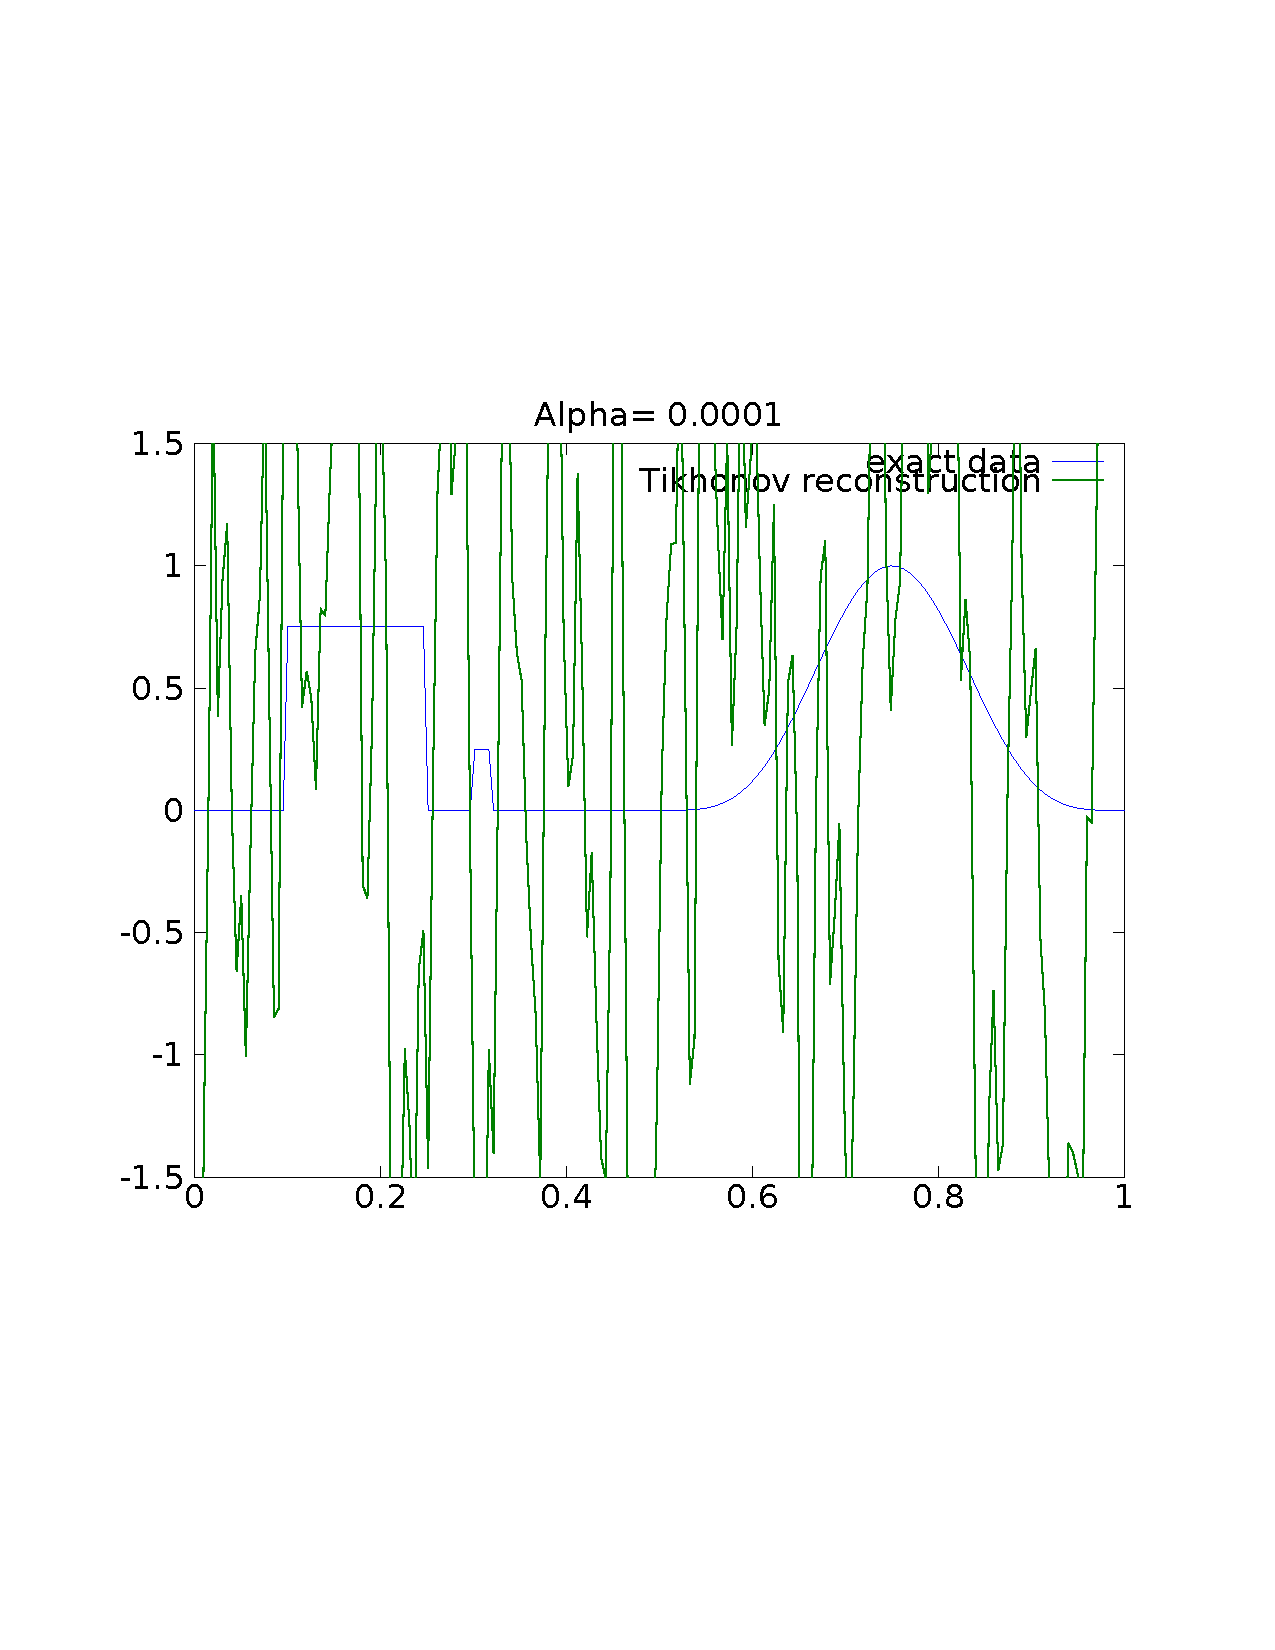
\includegraphics[width=\textwidth]{plots/reconstruct0001.pdf}
                \caption{$\alpha=0.0001$}
        \end{subfigure}%
        \begin{subfigure}[bh]{0.45\textwidth}
                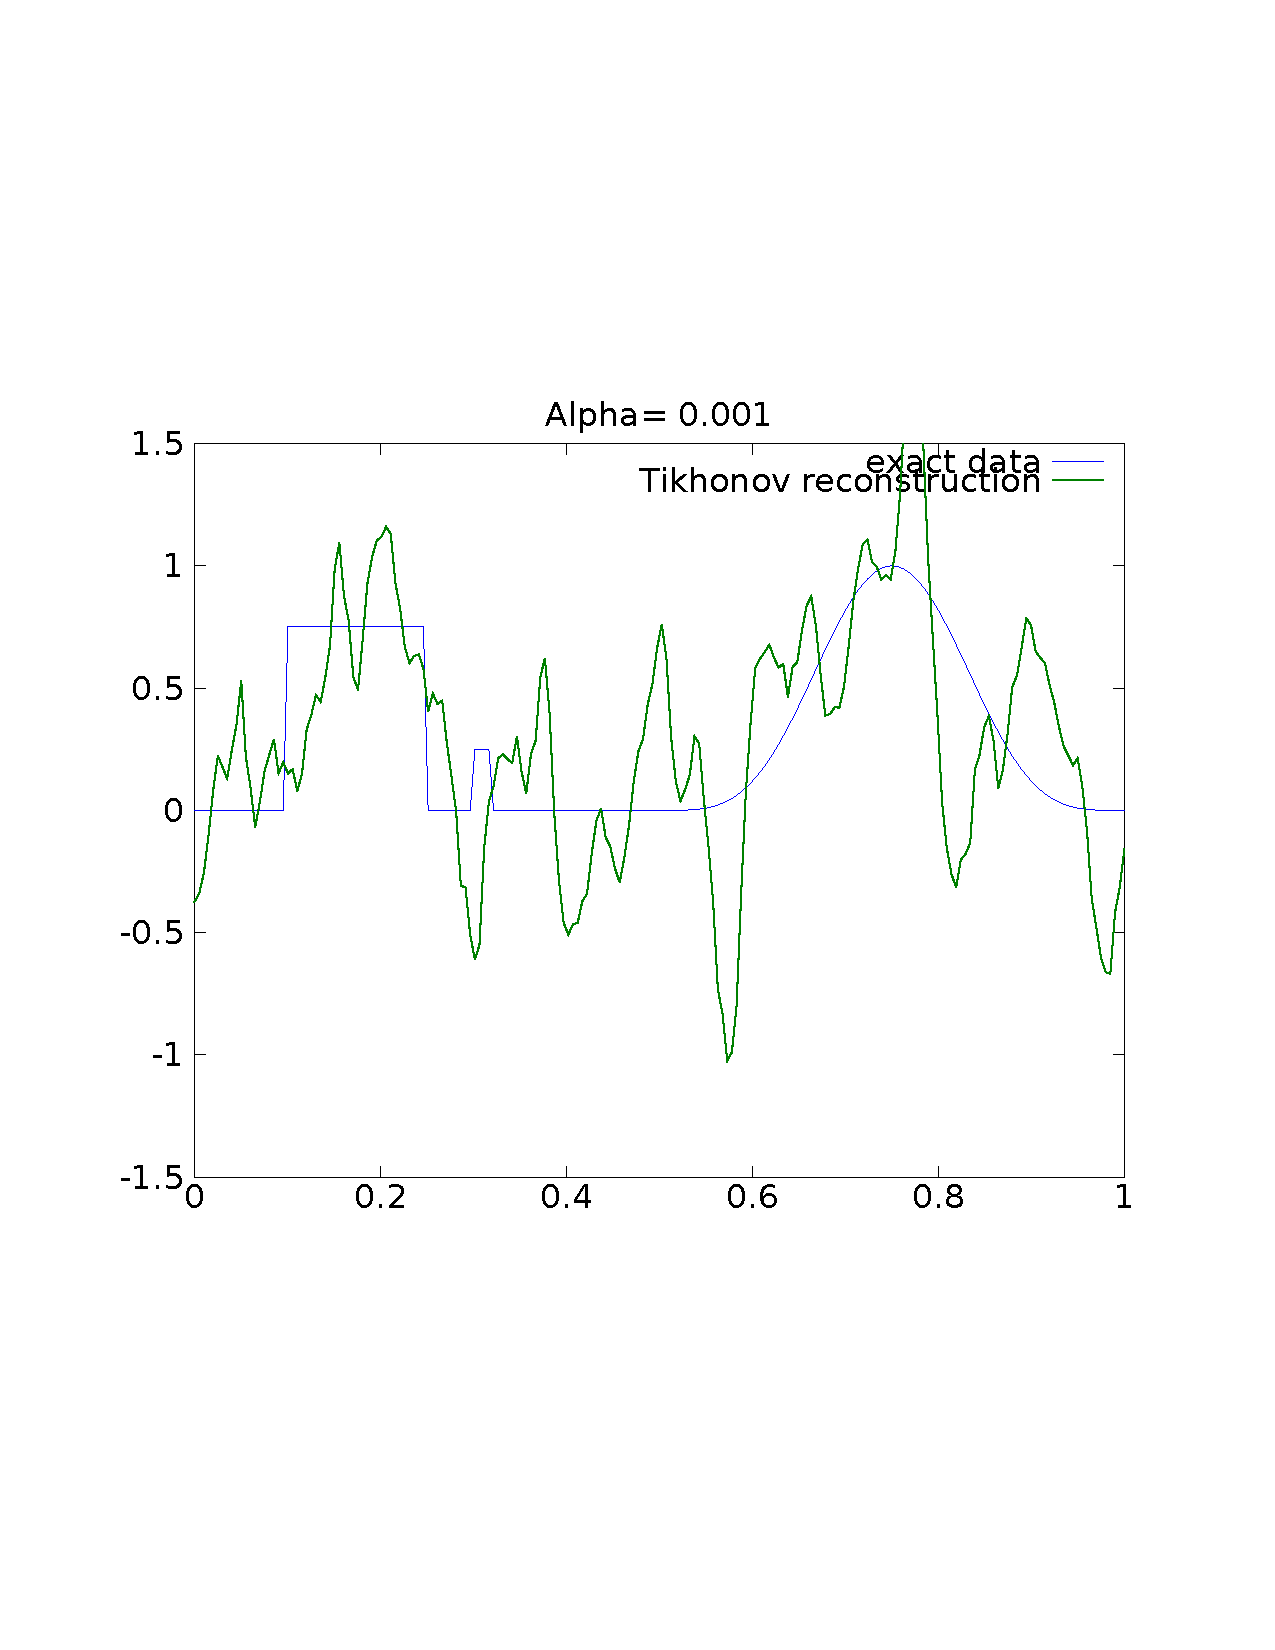
\includegraphics[width=\textwidth]{plots/reconstruct001.pdf}
                \caption{$\alpha=0.001$}
        \end{subfigure}
        \centering
        \begin{subfigure}[bh]{0.45\textwidth}
                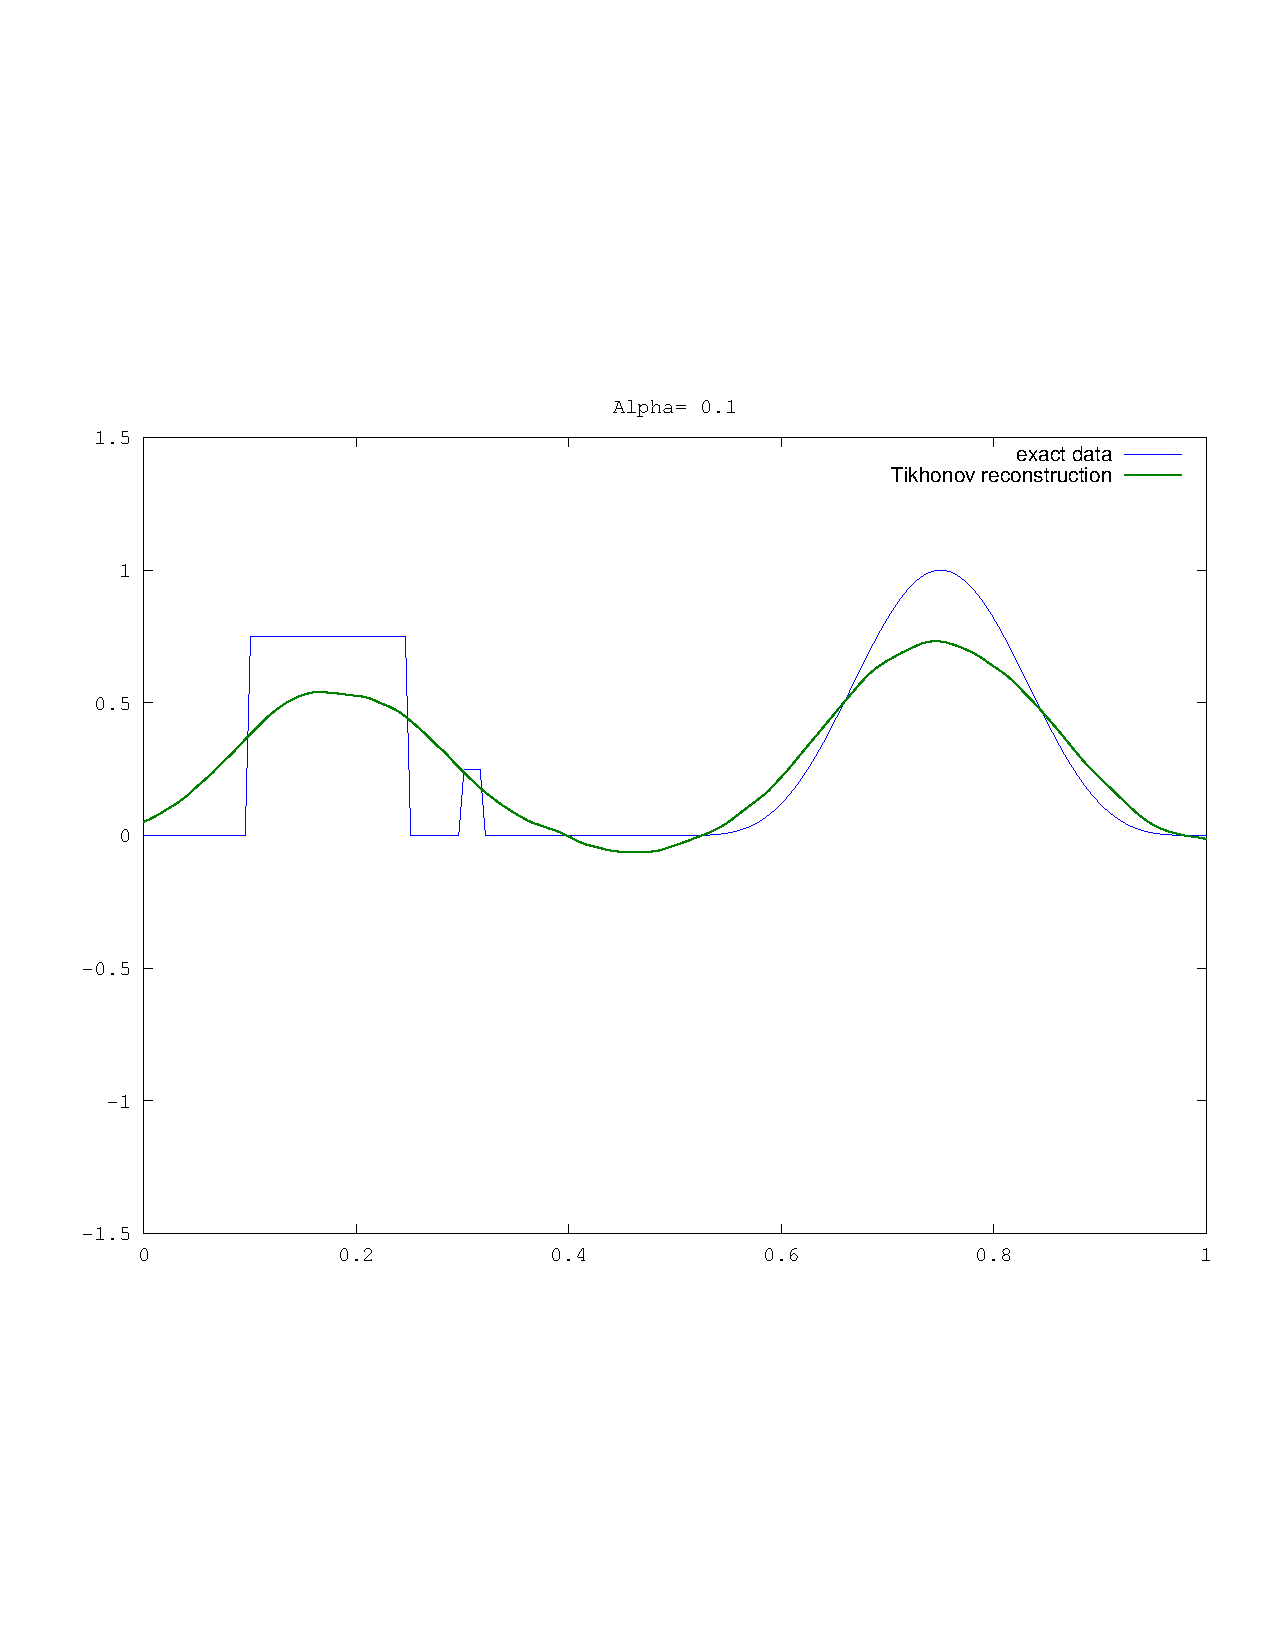
\includegraphics[width=\textwidth]{plots/reconstruct01.pdf}
                \caption{$\alpha=0.1$}
        \end{subfigure}%
        \begin{subfigure}[bh]{0.45\textwidth}
                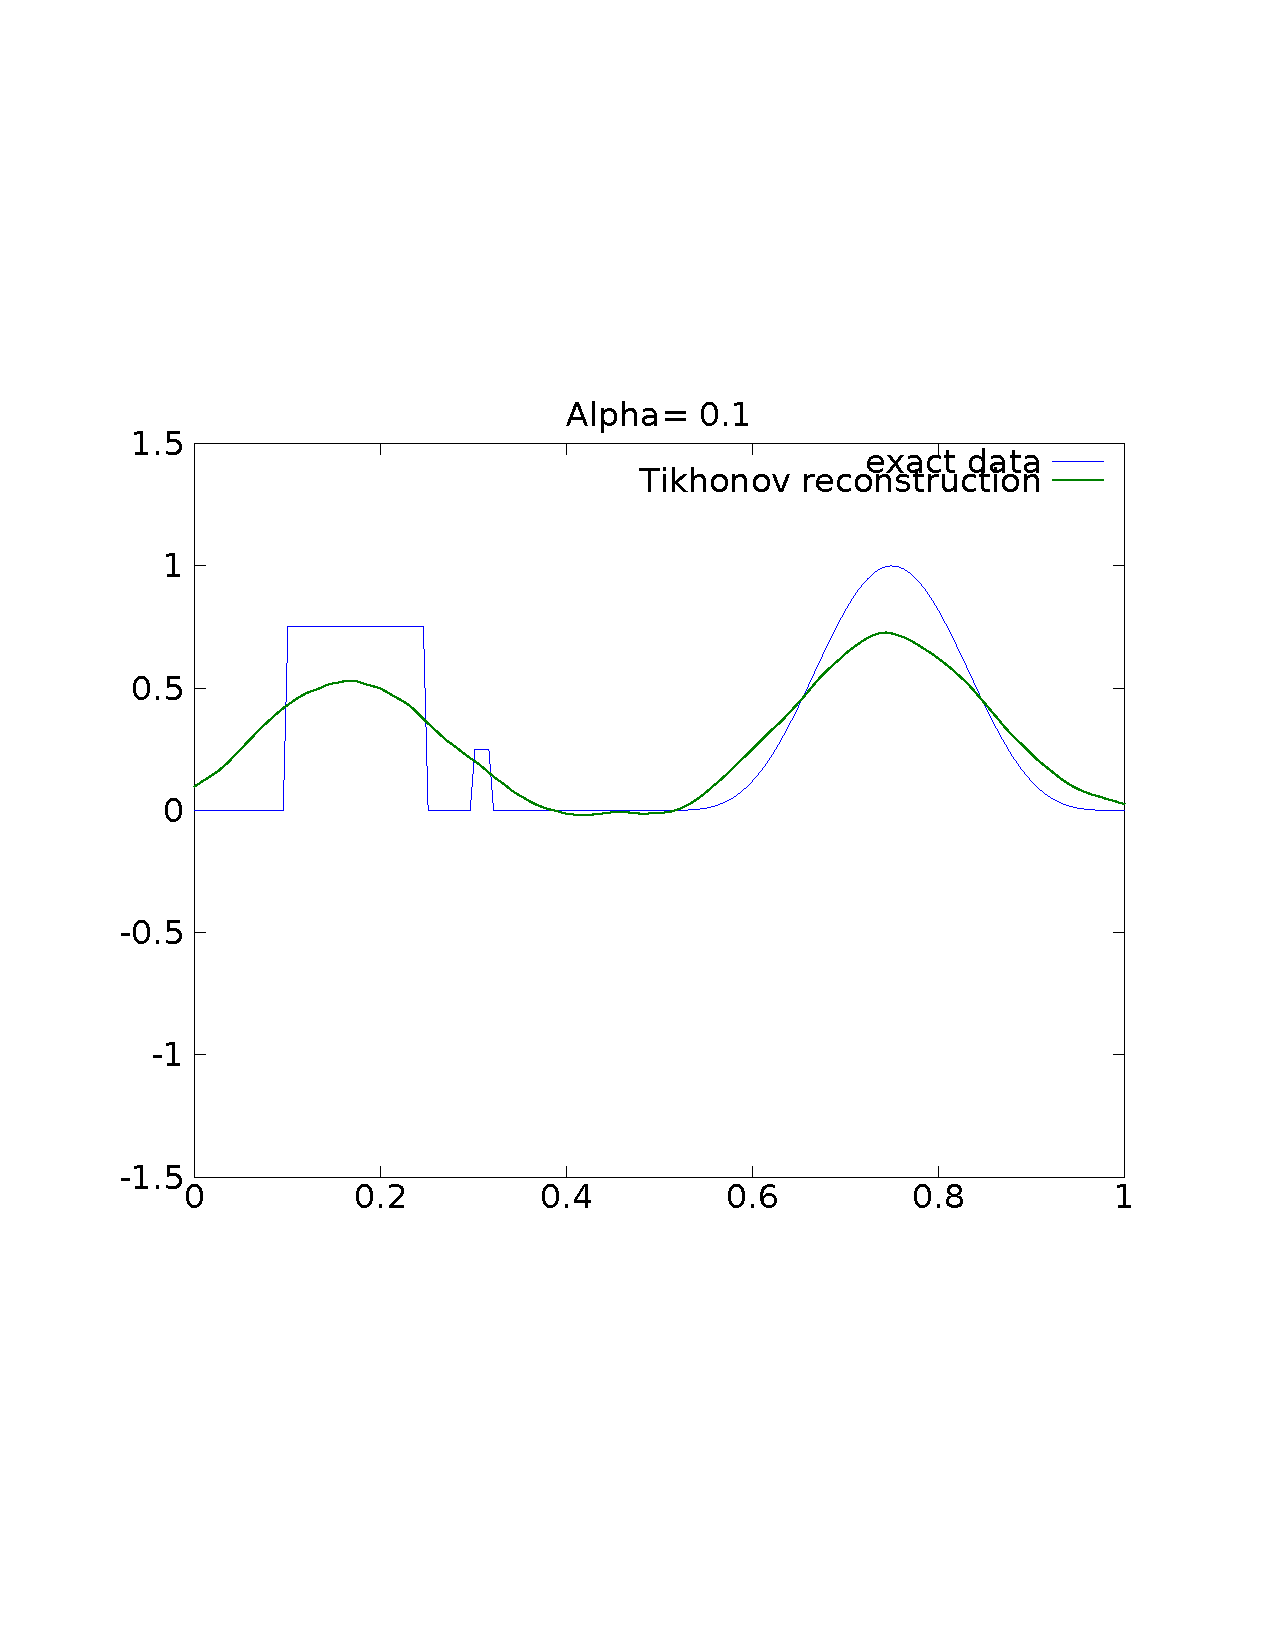
\includegraphics[width=\textwidth]{plots/reconstruct1.pdf}
                \caption{$\alpha=1.0$}
        \end{subfigure}
        \caption{Solutions to the inverse problem using Tikhanov
 regularization at varying values of $\alpha$.} 
 \label{fig:tik}
\end{figure}

Figure \ref{fig:tik} plots the solution to the inverse problem using
Tikhanov regularization at several different values of $\alpha$, the
regularization parameter.  

The Tikhanov filter is more sensitive, with (a) and (b) (low values of
$\alpha]$) completely being dominated by noise. None of the underlying
signal is regained, as all the high frequency content blown up and
dominating. 

For higher levels of the regularization parameter, we regain a solution
similar to in the TSVD cases, where we capture the underlying trend of
the data, but none of the sharp features. Also, the highest value of the
filter does not overwhelm the signal completely, as in the TSVD case,
which is interesting. 


\subsection{L-Curve}

\begin{figure}[!htb]
  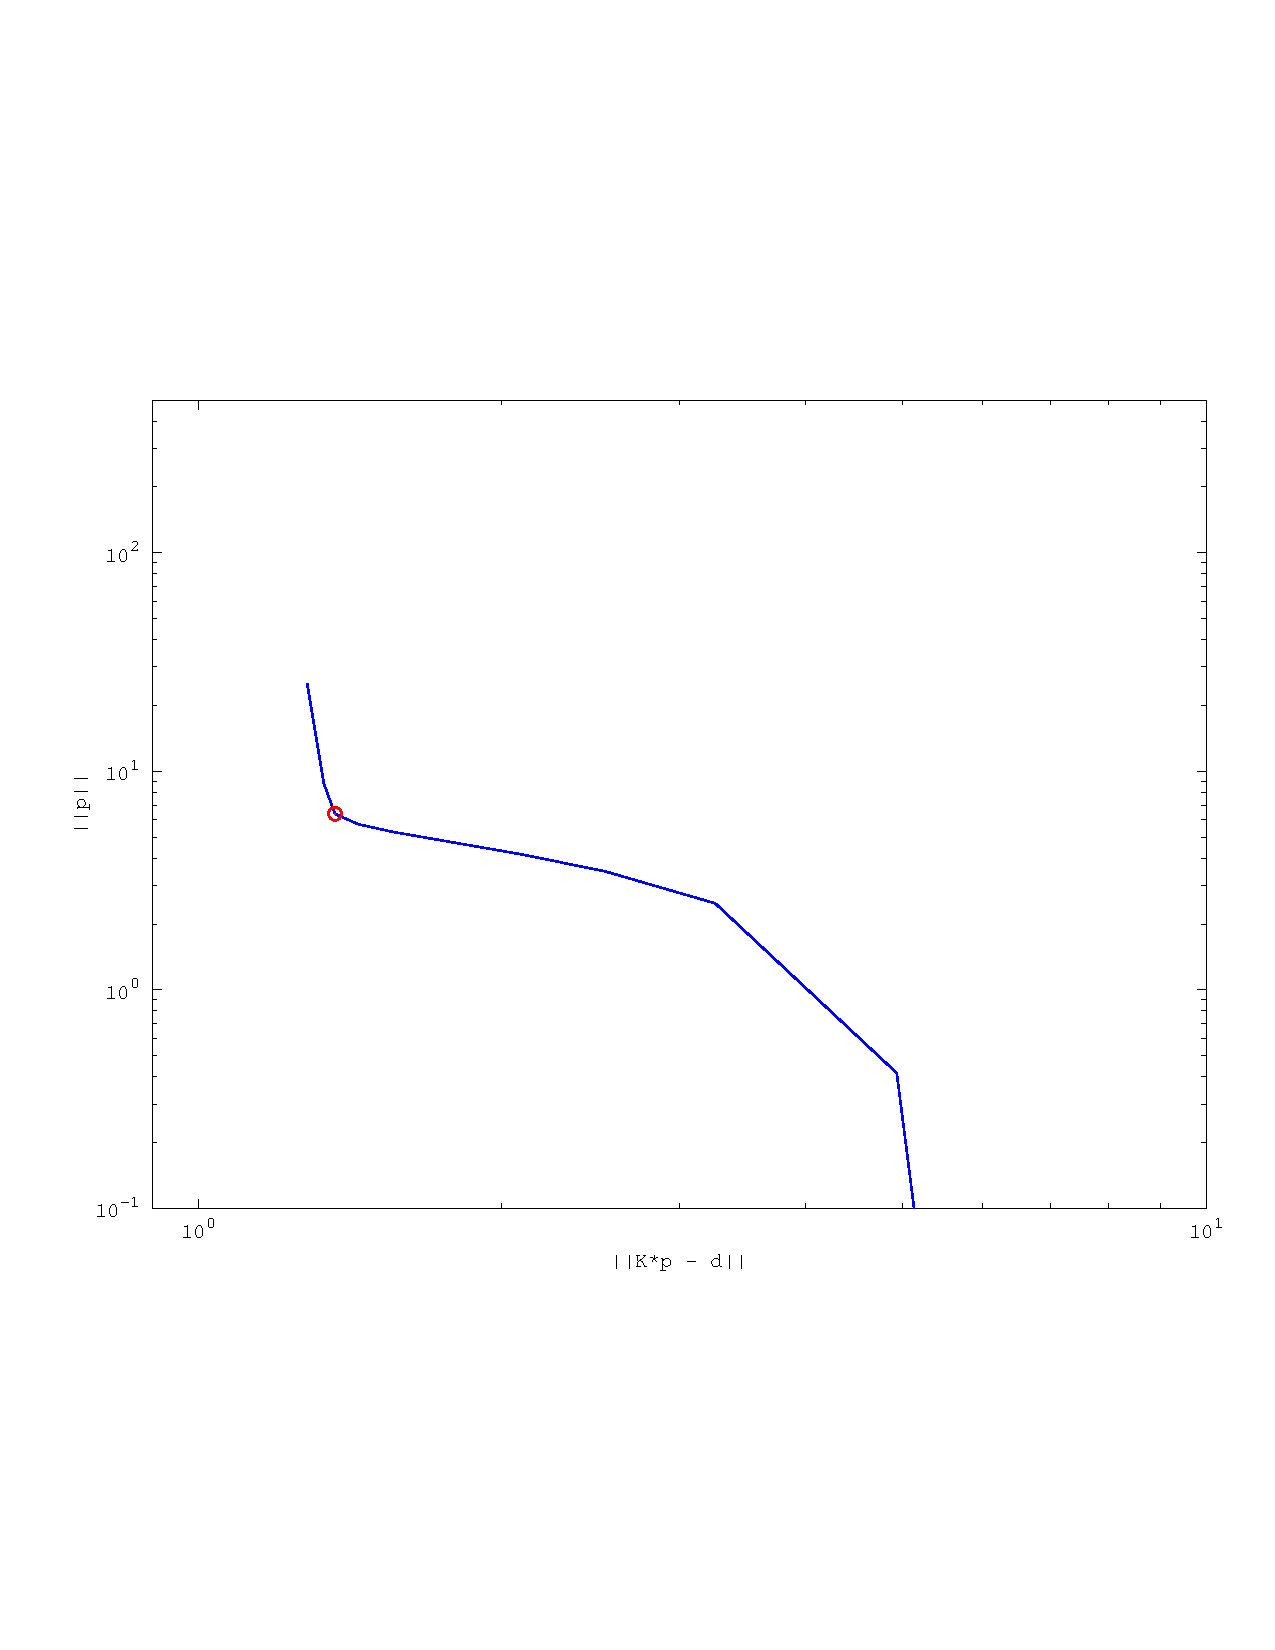
\includegraphics[scale=.6]{plots/L-curve.pdf}
  \caption{The L-curve} 
 \label{fig:lcurve}
\end{figure}

Figure \ref{fig:lcurve} plots the results of the L-curve criterion. The
red dot plotted is at 0.01. This is approximately the ``optimal'' value
of regularization, which is generally consistent with the observations
of the previous plots. 


\subsection{Morozov's Discrepancy Criterion}

\begin{figure}[!htb]
  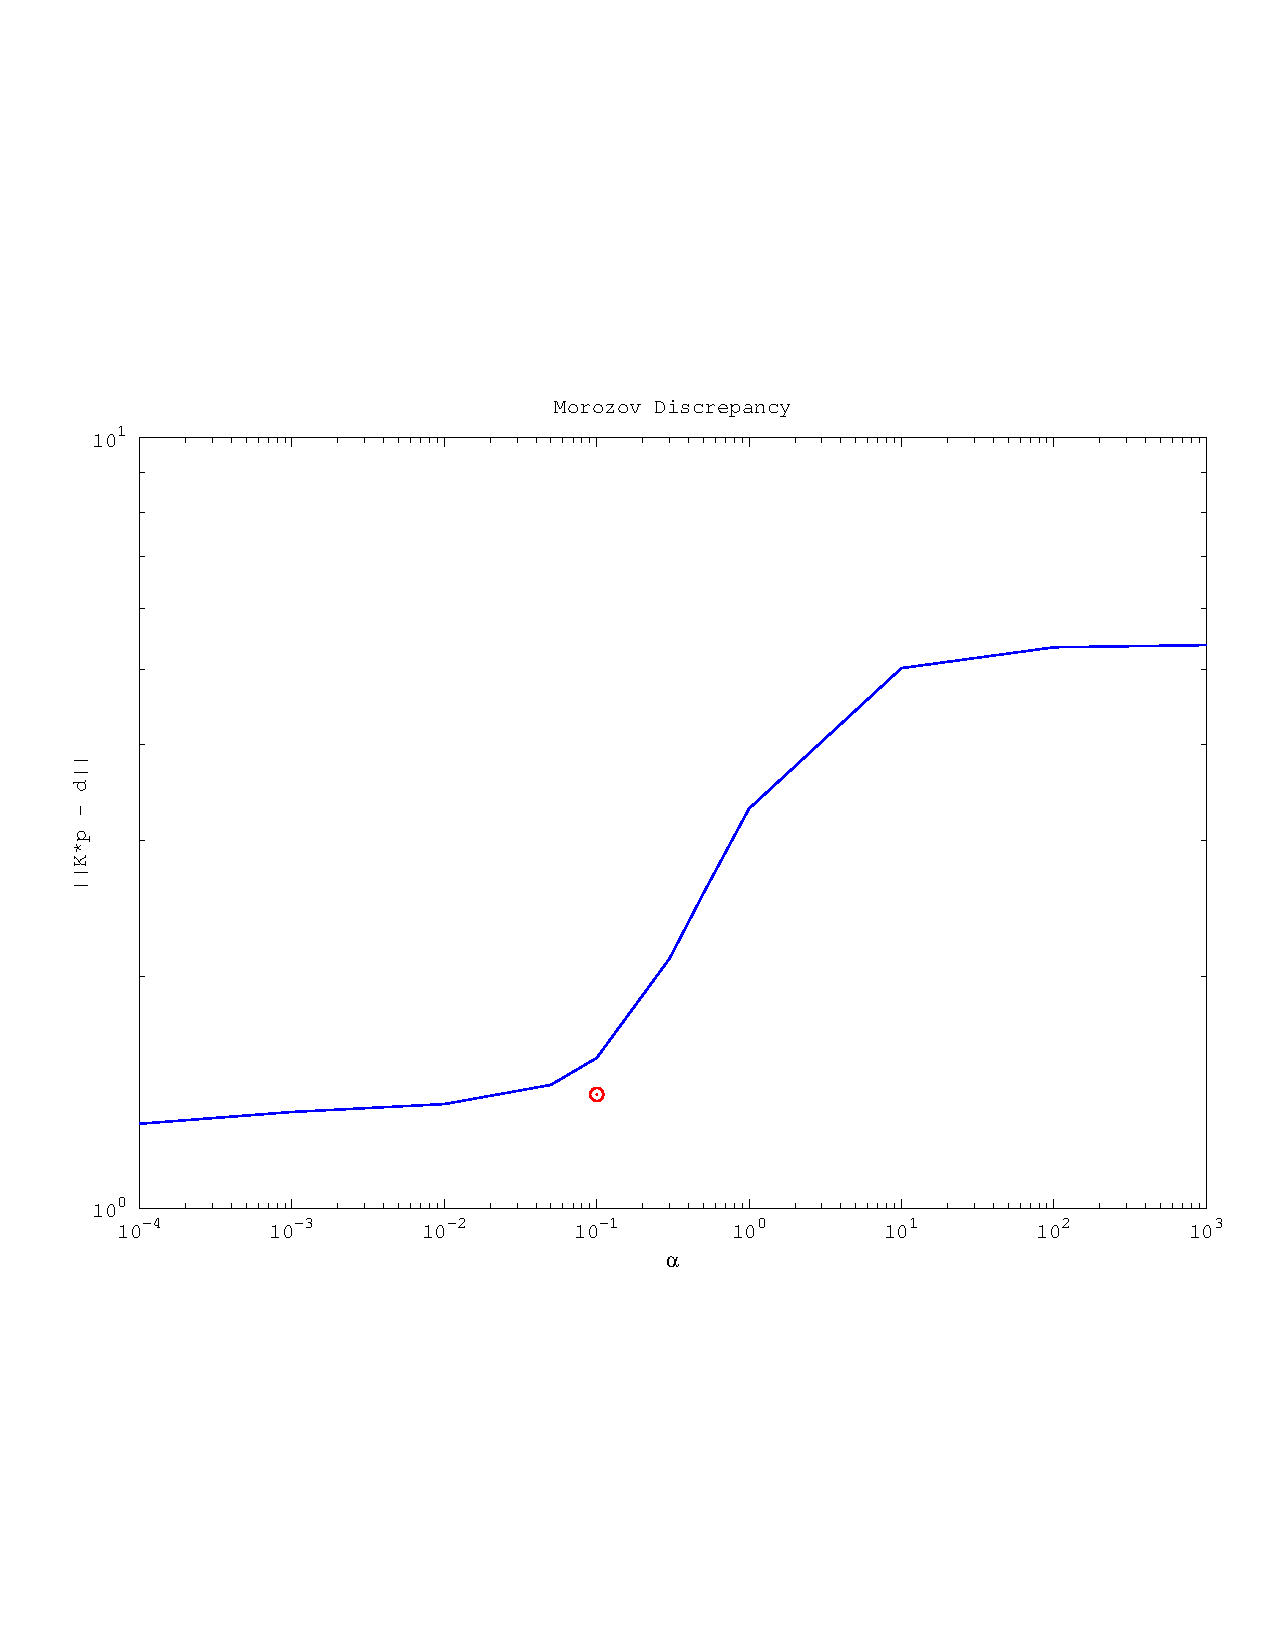
\includegraphics[scale=.5]{plots/morozov.pdf}
  \caption{Morozov discrepancy Criterion} 
 \label{fig:moro}
\end{figure}

Figure \ref{fig:moro} plots the results of Morozov discrepancy
criterion. I could not get the plots to draw a horizontal line, so that
red dot instead dictates the limit of $\delta$, the norm of the
error. This occurs at $\approx 4e-2$. This is smaller than the value
obtained using the L-curve, but not so much smaller that the value
appears suspect. 


\subsection{Actual Error}

\begin{figure}[!htb]
  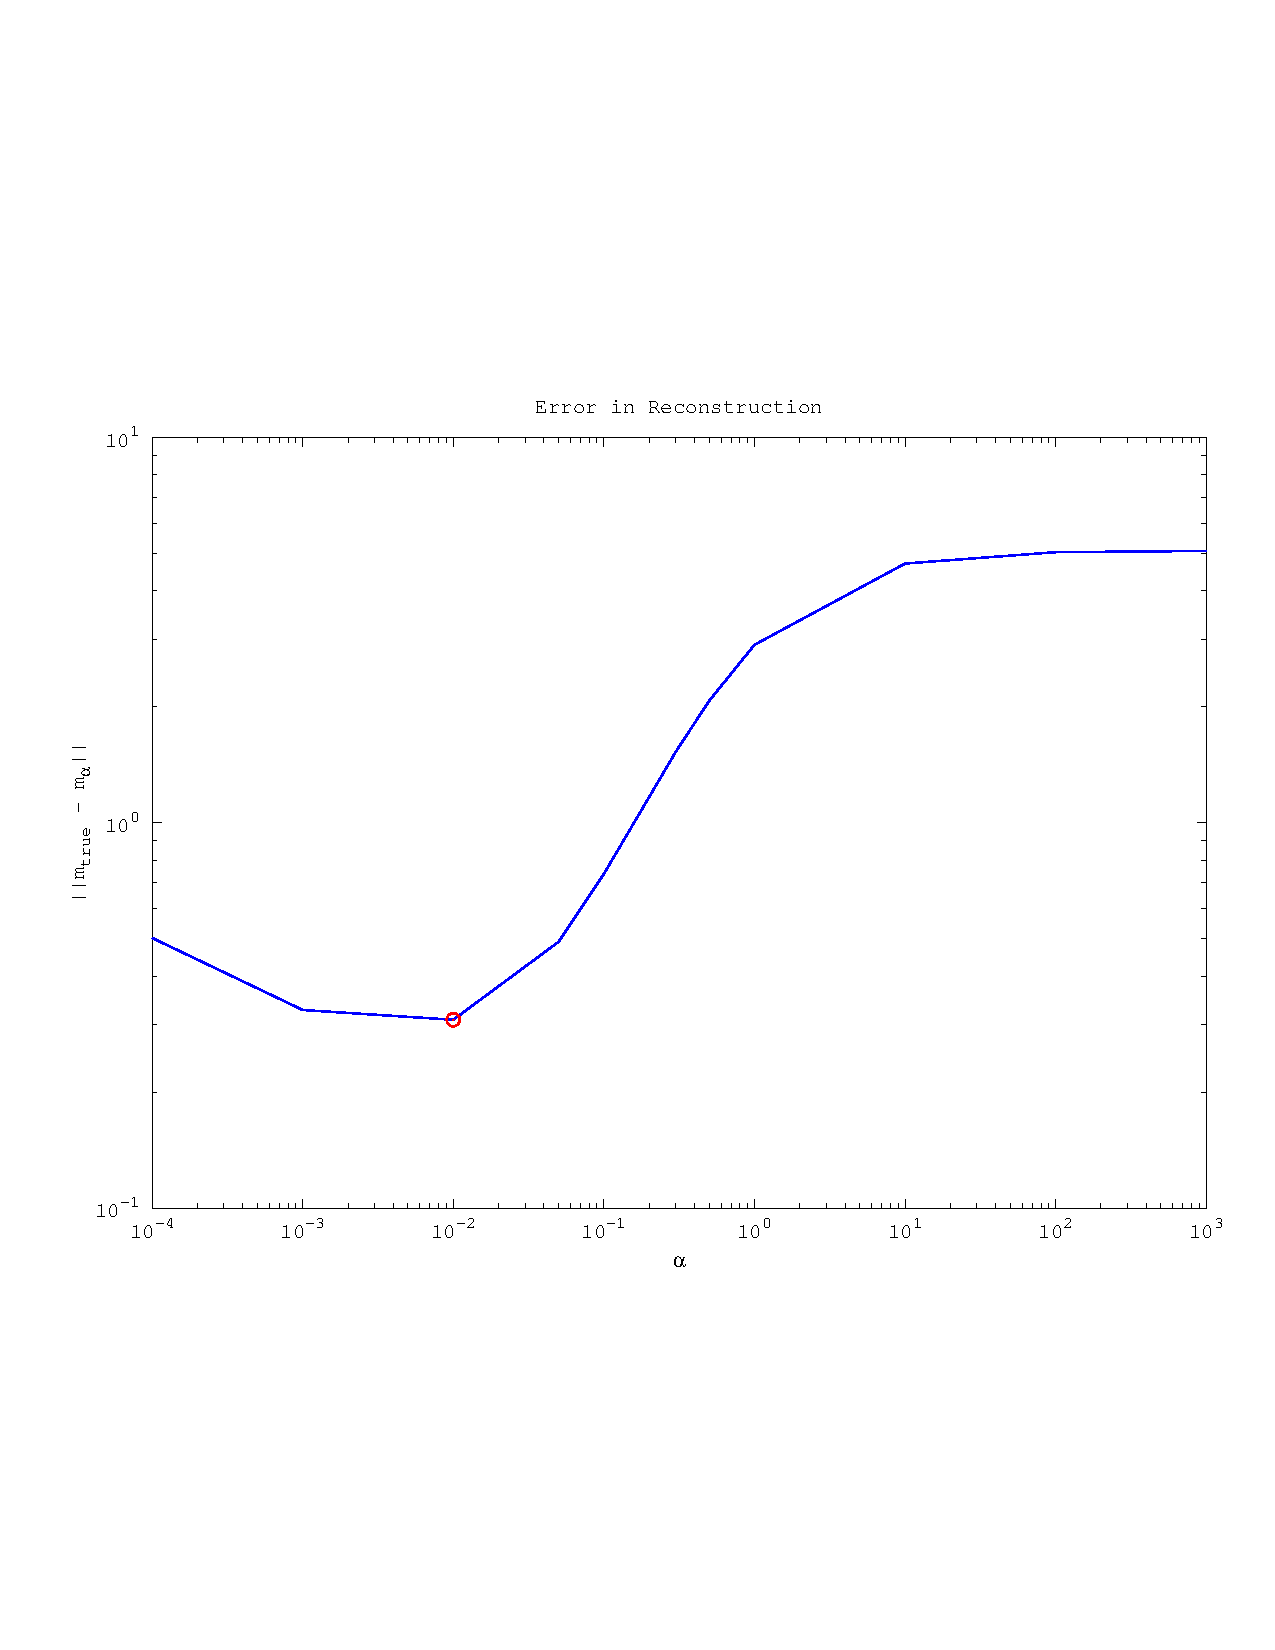
\includegraphics[scale=.5]{plots/true1d.pdf}
  \caption{The actual error in the reconstruction as a function of
 alpha. } 
 \label{fig:actual}
\end{figure}

Figure \ref{fig:actual} plots actual error in the reconstruction,
e.g. the norm of the difference between the reconstruction and the
actual (true) image, as a function of alpha. You can see that this
plot forms a rotated ``S'' curve, with the minimum occuring
approximately at the red dot. The value plotted is 0.01,
which actually agrees with the L-curve estimate. 

In any case, the values arrived at using the L-curve, Morozov's
discrepancy criterion and the actual error all agree within at least an
order of magnitude. So we are in the right ``ballpark''. As an aside, I
was actually quite pleased with the result, I would not have expected
these criterion to so closely arrive at values that are reasonable
guesses, even without knowledge of the true underlying signal. While
this is a toy problem, it does show that these criterion can be
effective means of approximating $\alpha$. Given the similarities
between the TSVD and Tikhanov, I would not be surprised to find that
these heuristics can be more generally useful for other regularizations as well. 


\newpage
\section{Problem 2}

% \begin{figure}[!htb]
%   
\includegraphics[scale=.5]{plots/longhorn.png}
%   \label{fig:true}
%   \caption{The true image.} 
% \end{figure}

% Figure \ref{fig:true} plots the true image, that we will be attempting
% to reconstruct through inversion. 

\subsection{Memory Requirement}

How much memory would be required to form the entire matrix, $K$?
We have $N^2$ model parameters. K lives in $\mathbb{R}^{N_2 * N_2}$. 
With $N=128$, then 
\begin{equation}
\frac{N^2 * N^2 * 8 \text{Bytes}}{(1024)^3} = 2 \text{GB}
\end{equation}
So while this is not inaccessible on modern HPC systems, it is certainly
not efficient.  

\subsection{L-Curve}

\begin{figure}[!htb]
  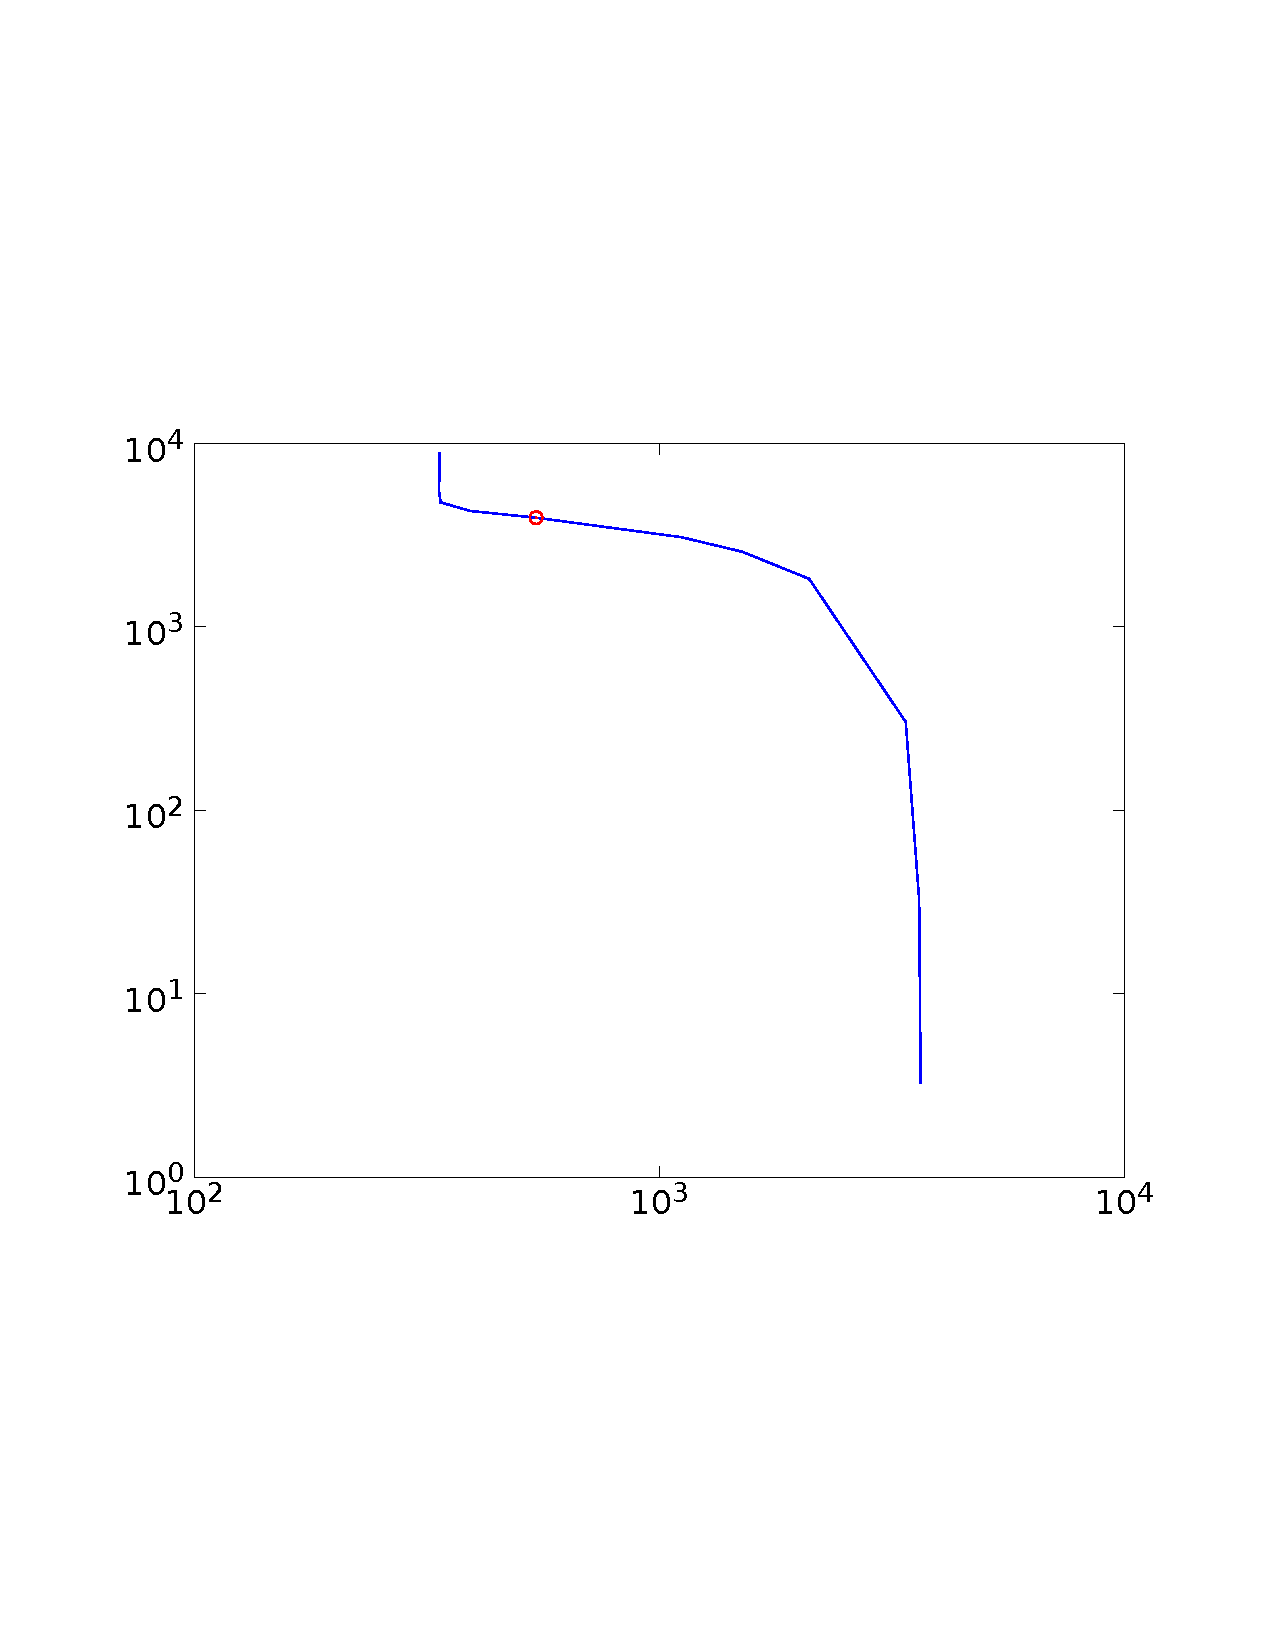
\includegraphics[scale=.5]{plots/L-curve2d.pdf}
  \caption{The L-curve for the 2d problem.} 
  \label{fig:l2d}
\end{figure}

Figure \ref{fig:l2d} plots the L-curve. The red dot is approximately at
the location of the optimal value of $\alpha$, which is found to be
$\approx 0.05 - 0.001$. 

\subsection{Actual Error}

\begin{figure}[!htb]
  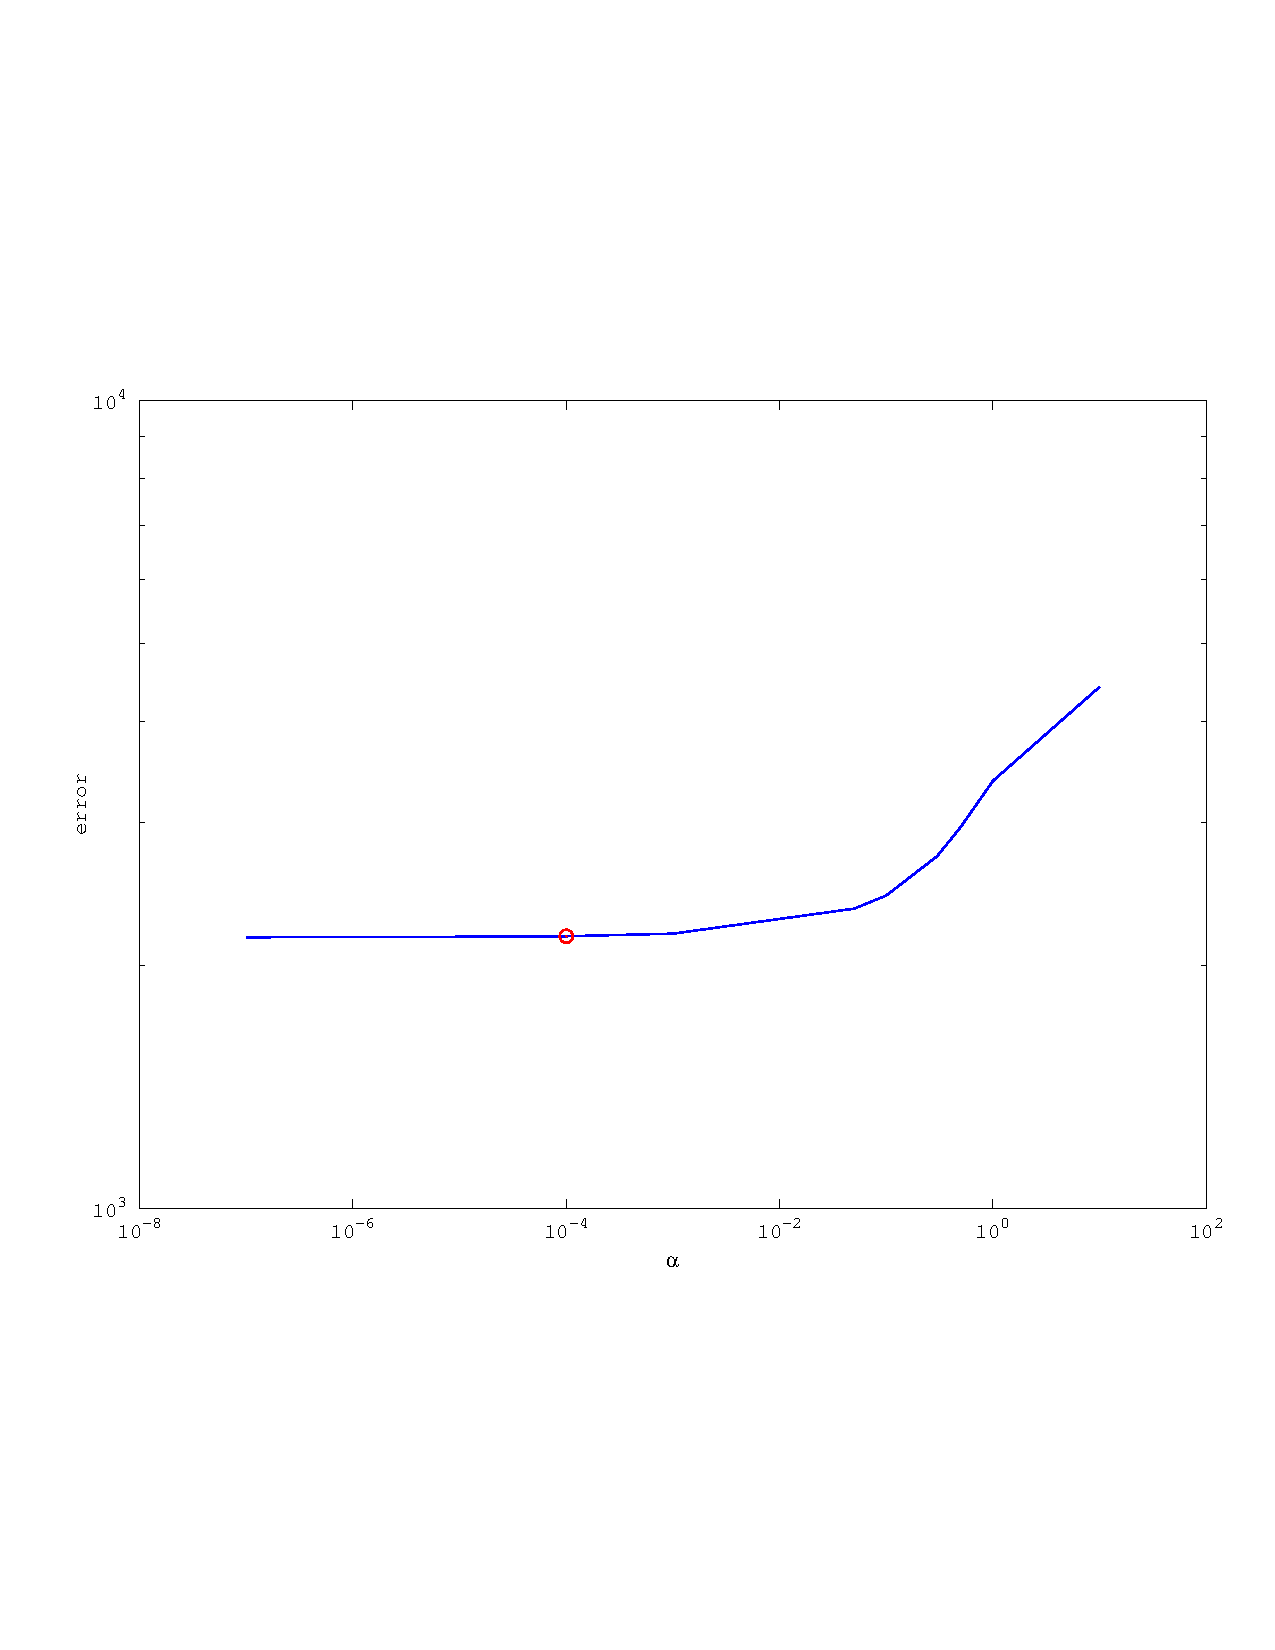
\includegraphics[scale=.5]{plots/2d-true.pdf}
  \caption{The actual error in the reconstruction as a function of
 alpha, for the 2d problem.} 
  \label{fig:2dt}
\end{figure}

Figure \ref{fig:2dt} plots the true error. Surprisingly, the error curve
appears to flatten out at lower values of alpha, implying a constant
error. Clearly any values less than $1e-3$ appear to be prefered, as the
error increases at higher values of $\alpha$. 

To calculate the error, I only needed to solve the conjugate gradient
(as before) and then calculate the norm of the misfit against $I$, the
true image:
\begin{lstlisting}
 I_alpha = pcg(@(in)apply(in,K1,K2,N1,N2,alpha),K_Ibn(:),1e-6,1500);
 misfit(k) = norm((K1 * (K2 * reshape(I_alpha,N2,N1))')' - I);        
\end{lstlisting}
\begin{figure}[!htb]
        \centering
        \begin{subfigure}[bh]{0.65\textwidth}
                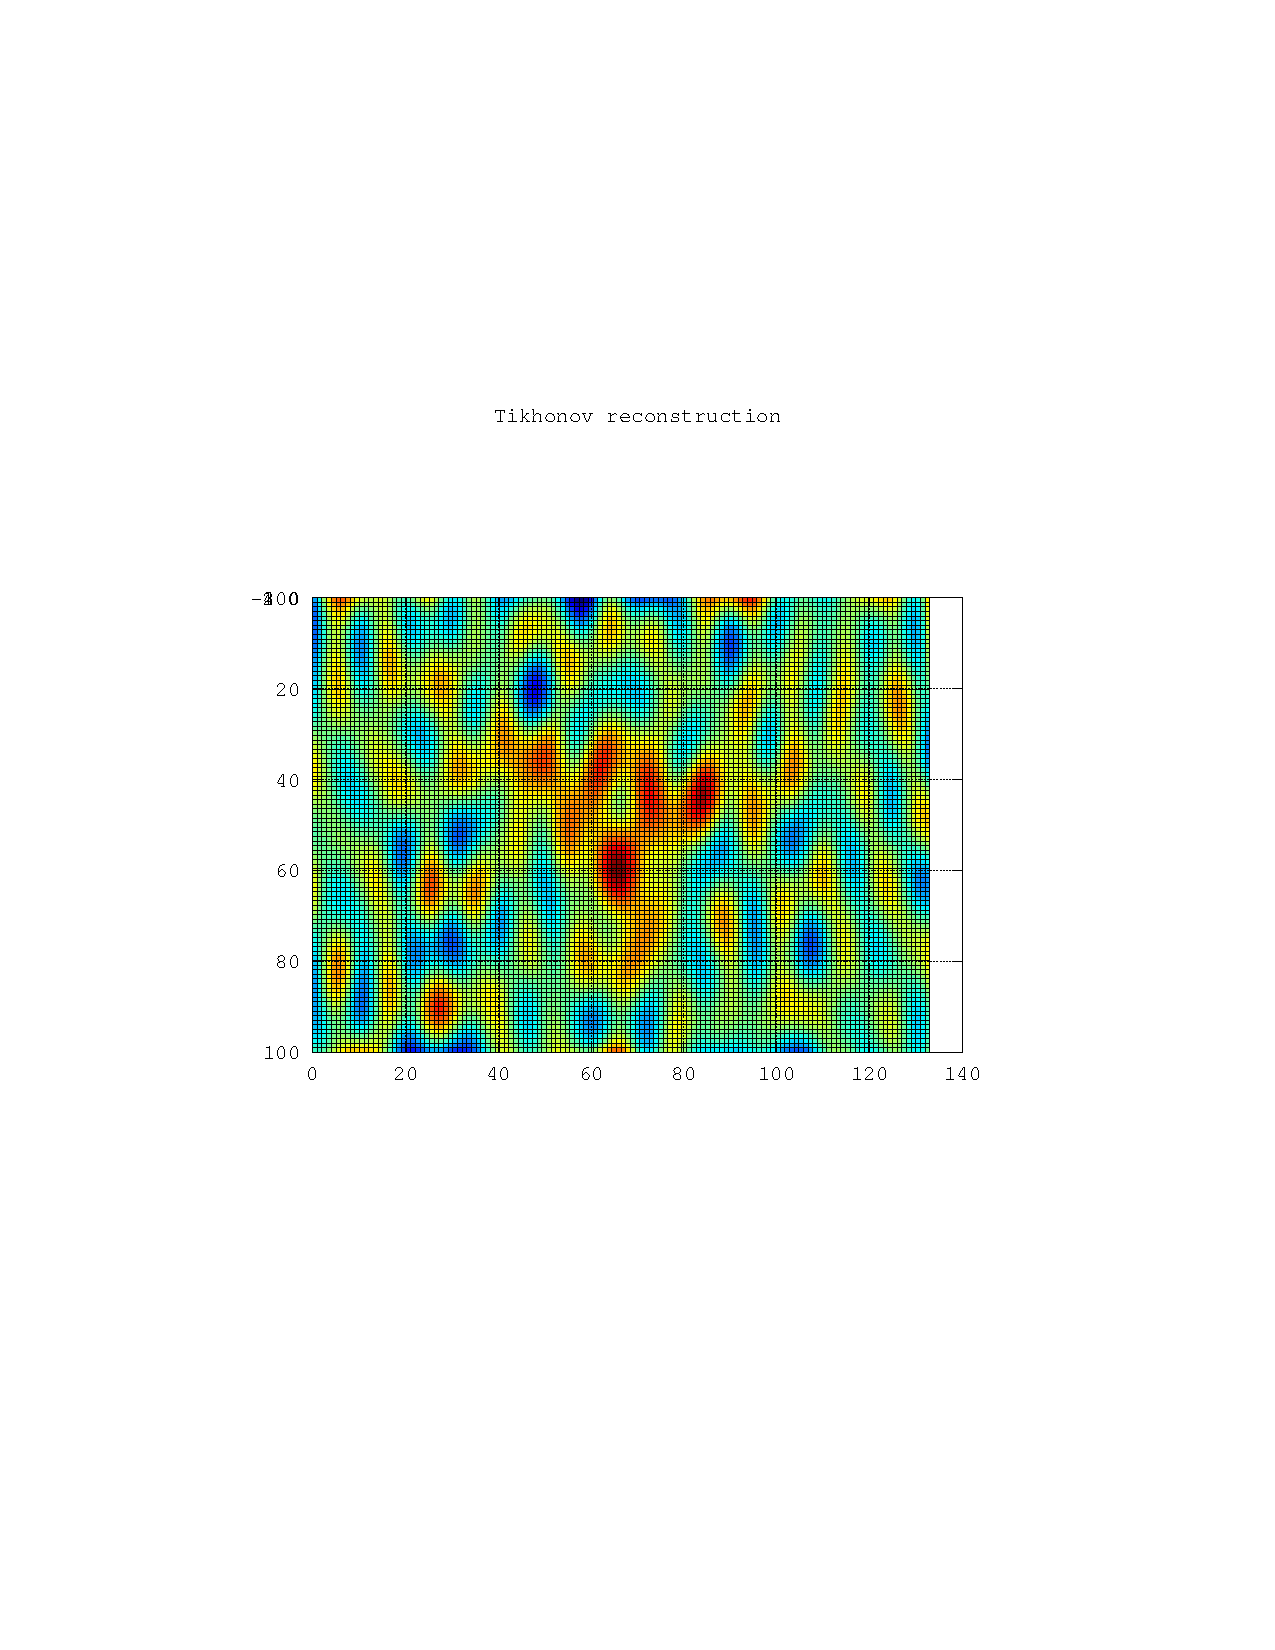
\includegraphics[width=\textwidth]{plots/tikrecon0001.pdf}
                \caption{$\alpha=0.0001$}
        \end{subfigure}%
        \begin{subfigure}[bh]{0.65\textwidth}
                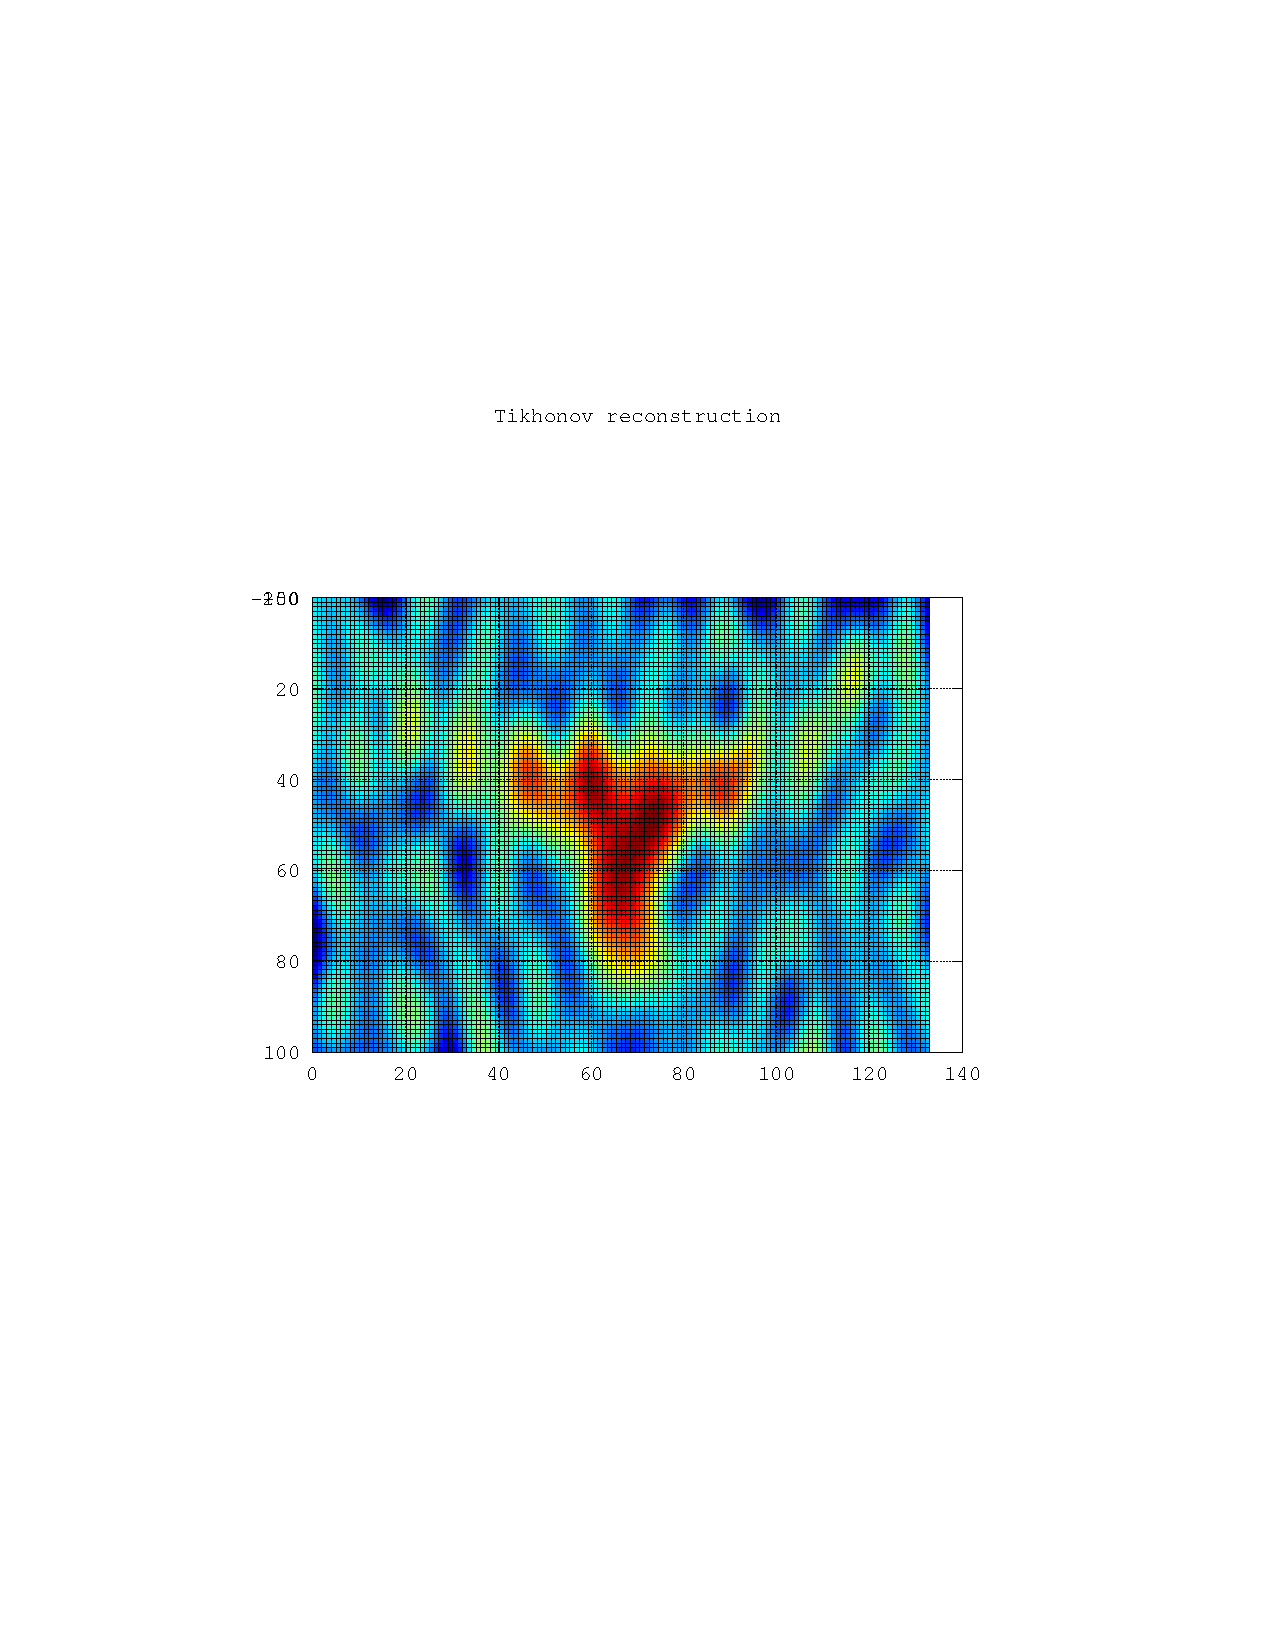
\includegraphics[width=\textwidth]{plots/tikrecon001.pdf}
                \caption{$\alpha=0.001$}
        \end{subfigure}
 \caption{The reconstructed image.}  
\label{fig:tik}
\end{figure}

The ``true'' image would imply then that the L-curve is too conservative
an estimate, and smaller values of $\alpha$ are acceptable. However, I
don't believe that. Figure 9 plots the Tikhanov
reconstruction for $\alpha = 0.001$ and $\alpha = 0.0001$. Clearly the
true image is recognizable in the right hand side, and not at all in the
left. So I believe that I either have a bug in my calculation of the
actual error, or the L-curve is, somehow, a more reliable estimate of
``good'' values of $\alpha$, here. 

\end{document}